% Neurocomputing submission --- Elsevier elsarticle format.
% NOTE: elsarticle is not installed on the local TeX here; this compiles on
% Overleaf (elsarticle is built in) or after `tlmgr install elsarticle` /
% `apt install texlive-publishers`. For the INITIAL submission, Elsevier's
% "Your Paper Your Way" also accepts the single cleanly-compiling PDF from main.tex.
\documentclass[preprint,12pt]{elsarticle}
% Scalable (Type 1) fonts with proper ToUnicode maps so ligatures (ff, fi, ffi)
% render and *copy/paste* correctly --- without this the default CM bitmap fonts
% drop ligatures on extraction ("tradeoff" -> "tradeo", "fixed" -> "xed").
\usepackage{lmodern}
\usepackage[T1]{fontenc}
\usepackage[utf8]{inputenc}
\usepackage[expansion=false]{microtype}
\usepackage{graphicx}
\usepackage{tikz}
\usetikzlibrary{shapes.geometric,arrows.meta,positioning}
\usepackage{amsmath,amssymb}
\usepackage{amsthm}
\newtheorem{proposition}{Proposition}
\newcommand{\OOFCATSHIFT}{1.9}  % mean |in-sample - OOF| Cat3-among-errors shift (pp); set from triage_oof
\usepackage{booktabs}
\usepackage{longtable}
\usepackage{url}
\usepackage[hidelinks]{hyperref}
\journal{Neurocomputing}

% --- Cross-class compatibility shims (sections are shared with the LLNCS main.tex) ---
% elsarticle appends a period to run-in \paragraph headings; our section sources
% already include the period, so suppress the class-added one to avoid "Heading..".
\makeatletter
\def\els@aparagraph[#1]#2{\elsparagraph[#1]{#2}}
\def\els@bparagraph#1{\elsparagraph*{#1}}
\makeatother
% elsarticle's appendix \ref already expands to "Appendix A"; \appref avoids the
% duplicated word ("Appendix Appendix B") that a literal "Appendix~\ref" produces.
\newcommand{\appref}[1]{\ref{#1}}

\begin{document}
\begin{frontmatter}

\title{Don't Oversample the Boundary: A Remedy Decomposition of the Minority
Deficit in Imbalanced Learning}

\author[a]{Cameron Hamilton\corref{cor}}
\ead{cameron@allianceai.co}
\cortext[cor]{Corresponding author.}
\affiliation[a]{organization={Alliance AI}}  % add city/country if desired

\begin{abstract}
Class imbalance is overwhelmingly handled by oversampling, yet SMOTE-family methods
typically trade majority-class accuracy for minority-class recall, and it is rarely
clear \emph{why} oversampling helps. We introduce a \emph{remedy decomposition} of
the misclassified minority: an out-of-bag error triage (ensemble confidence and
local class representation, validated against an aleatoric--epistemic uncertainty
decomposition) is combined with a threshold-recoverability test, assigning each
minority error to the remedy that would fix it: \emph{threshold-recoverable} (its
score already clears the tuned decision threshold; only the default cutoff is
wrong), \emph{data-reducible} (more same-class data would help), or
\emph{irreducible} (genuine class overlap). Across 79 real datasets the deficit is
predominantly threshold-recoverable (mean $68\%$; $80\%$ at imbalance ratio $>3$);
only $\sim$6\% is data-reducible and $\sim$17\% irreducible. This explains a known
but unexplained regularity: SMOTE-family resampling does not improve ranking (AUC
is unchanged) and a threshold move reproduces its benefit without synthetic
generation; single undertrained neural networks, whose ranking imbalance itself
corrupts, are the exception. On controlled mixtures with a
\emph{known} Bayes boundary, standard SMOTE places an overlap-dependent fraction of
synthetic points \emph{across} that boundary, and a short proposition shows why
interpolating boundary seeds crosses into majority-posterior space. Once every strategy receives
the same out-of-fold threshold tuning, the default-threshold gap between
non-generative and generative families collapses to within $\pm1$\,pp across three
base learners (against $+6.4$\,pp from tuning the threshold alone): the SMOTE
family's apparent edge is an operating-point effect, not a discrimination gain. The
practical conclusion: diagnose the deficit; for most of it, move the decision
rather than oversample.

\end{abstract}

\begin{keyword}
class imbalance \sep SMOTE \sep decision threshold \sep calibration
\sep uncertainty decomposition \sep data complexity
\end{keyword}

\end{frontmatter}

\section{Introduction}\label{sec:intro}

Class imbalance is a persistent challenge in machine learning. In production
settings the cost of the resulting performance degradation is not abstract: in
medical screening at 10\% prevalence, a one-percentage-point drop in specificity
at fixed sensitivity multiplies the false-positive volume that clinicians must
reconcile, and in fraud detection it directly inflates the analyst caseload that
determines operational feasibility. When one class dominates the training
distribution, classifiers tend to optimize for majority-class accuracy at the
expense of minority-class recall \cite{he2009learning}. SMOTE
\cite{chawla2002smote}, which generates synthetic minority instances by
interpolating between existing samples and their nearest neighbours, remains the
dominant solution after two decades and has spawned hundreds of variants
\cite{fernandez2018smote,kovacs2019smote}. Yet a stubborn regularity persists:
SMOTE variants almost invariably degrade majority-class accuracy while improving
minority-class recall. This accuracy--balanced-accuracy tradeoff is so common
that practitioners treat it as inherent to oversampling.

The field has responded in two ways. One line asks \emph{which} resampling
method a given dataset needs: data-complexity studies show that data
characteristics, not the imbalance ratio alone, moderate oversampling
effectiveness \cite{komorniczak2022data}, and meta-learning research recommends
a resampler from dataset meta-features
\cite{carvalho2025resampling,jiang2026beyond}. Another line has grown openly
critical: large benchmark studies find that oversampling often fails to
outperform doing nothing once evaluation is done carefully, and that reported
gains depend heavily on which metrics are chosen
\cite{tarawneh2022stop,elor2022smote}. Both lines are
\emph{correlational}: they relate measured data characteristics or benchmark
outcomes to observed performance, but do not explain \emph{why} a method helps
or harms, and the proposed selection rules barely beat the trivial ``always
SMOTE'' baseline. What is missing is a \emph{mechanistic} account of the
tradeoff that tells us which lever to pull.

We provide such a mechanistic account. We argue the tradeoff is \emph{not}
inherent to oversampling but
is a mechanistic consequence of \emph{where} SMOTE generates synthetic data.
Standard SMOTE uses every minority instance as an interpolation seed, including
those in regions of genuine class overlap near the decision boundary. Generating
there pushes the learned boundary into majority-class territory, recovering some
minority instances while misclassifying previously correct majority ones. We
establish this in two steps. On controlled Gaussian mixtures with a \emph{known}
Bayes boundary, standard SMOTE demonstrably places synthetic points \emph{across}
that boundary. On real data, where the boundary is unobserved, a controlled
interventional experiment manipulates \emph{where} synthetic points are generated:
augmenting \emph{only} the model-estimated boundary (irreducible) errors reproduces
the full SMOTE signature (balanced accuracy $p<0.001$, negative accuracy trend),
whereas augmenting non-boundary or random instances has no such effect. The
evidence indicates that much of the cost traces to \emph{where} synthetic data is
placed, rather than to rebalancing per se.

To localize this boundary/overlap region on real data we introduce \textbf{Error
Instance Triage}, which categorizes each misclassified training instance from
\emph{out-of-bag} random-forest confidence and local class representation; the
categories are interpreted through, and validated against, an
aleatoric--epistemic uncertainty decomposition
\cite{shaker2020aleatoric,hullermeier2021aleatoric}.
We state the scope plainly: the triage \emph{instrument} is computed from
random-forest ensembles (the standard vehicle for this decomposition
\cite{shaker2020aleatoric}), while the downstream conclusions are evaluated
across three base learners, gradient-boosted trees, random forests, and
logistic regression (\S\ref{sec:results:frontier}). The categories are:

\begin{enumerate}
\item \textbf{Cat\,1 (Noise):} likely mislabeled instances: high total but
  low aleatoric uncertainty; the label conflicts with the feature pattern.
\item \textbf{Cat\,2 (Data-limited):} errors in regions lacking same-class
  evidence: high epistemic uncertainty, low local class density. These are
  \emph{reducible}: more correct-class data would resolve them.
\item \textbf{Cat\,3 (Irreducible):} errors in estimated boundary/overlap regions
  where classes overlap: high aleatoric uncertainty. These are \emph{not}
  reducible by adding data.
\end{enumerate}

The decomposition yields a diagnostic, not a new oversampler. On real imbalanced
data the misclassified minority concentrates in these estimated boundary/overlap
regions (Cat\,3 is $\sim$85\% of errors, a fraction that is stable under strict
out-of-fold re-estimation), exactly where SMOTE's harm originates. Yet that
balanced-accuracy deficit turns out to be largely a \emph{decision-threshold
artefact}: moving the decision threshold alone (a non-generative change)
recovers roughly nine percentage points of balanced accuracy over the default
threshold (\S\ref{sec:results:frontier}), without any synthetic generation. The practical implication is that the lever is
the \emph{decision rule}, not synthetic generation, and indeed non-generative
strategies (threshold-moving, cost-sensitive learning, balanced ensembles)
capture the recoverable balanced accuracy \emph{without} the boundary-generation
accuracy cost.

We make this precise with a \emph{remedy decomposition} of the misclassified
minority that sorts each error into threshold-recoverable, data-reducible
(epistemic), or irreducible (aleatoric). We find the deficit is overwhelmingly
\textbf{threshold-recoverable} (mean $68\%$ across 79 datasets, $80\%$ at
$\mathrm{IR}>3$): the classifier's scores already place these instances above a
tuned operating point. The known
``move the threshold'' equivalence
\cite{provost2000imbalanced,elkan2001foundations,elor2022smote,goorbergh2022harm}
is the consequence: across a 16-strategy menu oversampling yields no ranking gain
and shifts the class prior in probability space rather than improving
calibration, and once \emph{every} strategy is given the same
out-of-fold threshold tuning the large default-threshold gap between the families
collapses to within $\pm1$\,pp across three base learners.
We turn the diagnosis into a prescription with a regime map and an
honestly-scoped selector, which beats the always-SMOTE / imbalance-ratio
paradigm, but only because the menu now includes the dominant non-generative
strategies, while a strong non-generative default is itself near-optimal.

\paragraph{Contributions.}
\begin{enumerate}
\item \textbf{A remedy decomposition of the minority deficit (headline).} We
  decompose the \emph{misclassified} minority by combining an error triage
  (out-of-bag confidence and local representation, validated against an
  aleatoric--epistemic uncertainty decomposition) with a threshold-recoverability
  test, mapping each error to the remedy that would fix it:
  \emph{threshold-recoverable}, \emph{data-reducible} (epistemic), or
  \emph{irreducible} (aleatoric). Unlike prior
  instance taxonomies, which score \emph{difficulty}
  \cite{napierala2016types,smith2014instance,swayamdipta2020dataset,seedat2022dataiq},
  ours conditions on the model being wrong and introduces the threshold-recoverable
  axis. Empirically the deficit is overwhelmingly threshold-recoverable
  ($68\%$ on average, $80\%$ at $\mathrm{IR}>3$).
\item \textbf{A mechanism behind the ``move the threshold'' equivalence.} The
  decomposition \emph{explains} a known regularity (that resampling does not
  improve ranking and a threshold shift reproduces its benefit
  \cite{provost2000imbalanced,elkan2001foundations,elor2022smote,goorbergh2022harm})
  by showing the deficit is mostly a thresholding artefact, so oversampling is
  an implicit, inefficient enactment of a threshold move. We give the geometric
  mechanism: on controlled mixtures with a \emph{known} boundary, SMOTE generates
  across it, and a short proposition (\S\ref{sec:method:theory}) shows why
  interpolating boundary seeds crosses into the majority-posterior region.
\item \textbf{Evidence at scale (confirmation, not claim).} Across 79 datasets and
  a 16-strategy menu we reproduce, on a broad roster, that oversampling yields no
  discrimination gain (AUC unchanged) and enacts a prior shift in probability
  space rather than a calibration improvement, and that once
  \emph{every} strategy receives the same out-of-fold threshold tuning, the
  $+5.76$\,pp default-threshold gap between the families collapses to within
  $\pm1$\,pp across three base learners (six evaluated; the documented exception
  is the single MLP, whose \emph{ranking} imbalance corrupts and resampling
  partially repairs, \S\ref{sec:results:frontier}). The apparent dominance of non-generative
  methods at the default threshold is an operating-point effect. We frame these as confirmation of
  \cite{elor2022smote,goorbergh2022harm,dalpozzolo2015calibrating} at scale.
\item \textbf{An honestly-scoped prescription.} The decomposition says which remedy
  applies; we add a regime map and, as a secondary analysis, a held-out selector
  that beats always-SMOTE by $3.5$ points, but an imbalance-ratio-only rule
  matches it and a strong non-generative default is near-optimal, so the
  \emph{menu}, not selector sophistication, is the lever (the practical answer to
  the selection problem left open by \cite{jiang2026beyond}).
\end{enumerate}

\section{Related Work}\label{sec:related}

\paragraph{Instance categorization for imbalanced learning.}
Several frameworks decompose training data by learning difficulty.
Instance Hardness \cite{smith2014instance} assigns a difficulty score per
instance from majority votes across multiple learners. Dataset Cartography
\cite{swayamdipta2020dataset} maps instances by training-dynamics
confidence/variability. Data-IQ \cite{seedat2022dataiq} extends this to
tabular data via prediction trajectories. The closest line of work is
Napiera{\l}a \& Stefanowski \cite{napierala2010learning,napierala2016types},
who categorize minority instances into safe, borderline, rare, and outlier
based on the proportion of same-class neighbours in a k-nearest-neighbour
graph; S\'aez et al.\ \cite{saez2016analyzing} extend this to multi-class
imbalanced data and analyze how oversampling interacts with each type. Crucially,
all of these characterize instance \emph{difficulty}; none condition on the model
being \emph{wrong} and ask \emph{which remedy applies}. Our decomposition differs
in three ways: (i) it operates on the \emph{misclassified minority} and maps each
error to a remedy --- move the threshold, add data, or accept it --- rather than
scoring difficulty; (ii) it introduces a \emph{threshold-recoverable} class (the
model already ranks the instance correctly and only the default cutoff is wrong),
an axis absent from prior difficulty taxonomies; and (iii) it combines a
model-based aleatoric--epistemic decomposition --- separating Bayes-rate ambiguity
from sample-size limits, which k-NN typing cannot --- with a local class-ratio
measure, used as a diagnostic rather than as a competing oversampler.

\paragraph{Threshold-moving, cost-sensitivity, and the limits of resampling.}
A long line of work argues the decision threshold, not the training distribution,
is the right lever under imbalance. Provost \cite{provost2000imbalanced} warns
against the default $0.5$ cutoff, and Elkan \cite{elkan2001foundations} shows that
changing class proportions is \emph{equivalent} to changing the decision
threshold/costs, so rebalancing barely alters the learned scoring function;
Drummond and Holte \cite{drummond2003c45} reach the analogous conclusion via cost
curves. Large-scale and clinical studies confirm the empirical consequence:
resampling does not improve ranking/AUC and its apparent gains are reproduced by a
threshold shift, while it degrades probability calibration
\cite{elor2022smote,goorbergh2022harm,dalpozzolo2015calibrating,carriero2025harms}.
We do \emph{not} claim these regularities as new --- we reproduce them across our
roster and instead \emph{explain} them: our reducibility decomposition shows the
misclassified minority is predominantly \emph{threshold-recoverable}, which is
\emph{why} a threshold move suffices and oversampling behaves as an implicit,
inefficient enactment of it. Our contribution is the per-instance instrument that
accounts for this equivalence and locates its exceptions (the data-reducible and
irreducible minority), not the equivalence itself.

\paragraph{Class overlap and imbalance.}
Santos et al.\ \cite{santos2023unifying} provide a unifying multi-view
panorama of the relationship between class overlap and class imbalance,
arguing that overlap is often the underlying driver of imbalance-related
difficulty. Their framing supports our boundary-generation diagnosis: when
SMOTE generates near class-overlap regions, the harm to accuracy is a
predictable consequence of overlap-blind seeding.

\paragraph{Characteristic-driven and complexity-guided selection.}
Komorniczak, Ksieniewicz, and Wo{\'z}niak \cite{komorniczak2022data}
demonstrate that data-complexity metrics correlate with the accuracy gain
oversampling delivers, and Carvalho et al.\ \cite{carvalho2025resampling} survey
how resampler performance tracks data structure. Most directly, Jiang and Ye
\cite{jiang2026beyond} control the imbalance ratio and show data characteristics
moderate oversampler choice --- yet their resulting selection rule does \emph{not}
beat always-SMOTE, and they leave open whether a held-out, characteristic-driven
selector can. This line is \emph{correlational}: it relates measured complexity to
observed performance without explaining the mechanism. Our contribution is
orthogonal --- a mechanism-level account of \emph{why} boundary generation hurts --- and we
answer the open selection question directly, on a full strategy menu with held-out
validation (\S\ref{sec:results:selection}), finding that the menu, not the
selector, is the dominant lever. Our account is mechanism-level and
intervention-supported rather than correlational.

\paragraph{SMOTE variants and cleaning.}
Borderline-SMOTE \cite{han2005borderline} restricts generation to instances
near the decision boundary; ADASYN \cite{he2008adasyn} upweights generation
in sparse minority regions. Both methods \emph{increase} generation in
exactly the regions we identify as harmful. Safe-Level-SMOTE
\cite{bunkhumpornpat2009safe} uses each seed's ``safe level'' (count of
same-class neighbours) to gate interpolation, an idea closely related to
ours but instantiated via k-NN heuristics rather than uncertainty
decomposition; we compare directly in \S\ref{sec:results}.
Post-hoc cleaning methods combine SMOTE with instance removal: SMOTE+ENN
\cite{batista2004study,wilson1972asymptotic} removes instances misclassified
by edited nearest neighbours, while SMOTE+Tomek
\cite{batista2004study,tomek1976two} removes Tomek-link pairs. These methods
are agnostic to \emph{why} an instance is problematic, removing both
correctable and boundary instances indiscriminately. Beyond the canonical
family, MWMOTE \cite{barua2014mwmote}, ProWSyn \cite{barua2011prowsyn}, and
polynomial-fitting SMOTE \cite{gazzah2008new} represent more recent
extensions. The 85-variant survey of Kov\'acs \cite{kovacs2019smote}
provides a broader perspective; we include the top three of his ranked
variants as baselines. Theoretically, Sakho et al.\ \cite{sakho2024rebalancing}
show that \emph{default} SMOTE asymptotically copies minority points and that its
synthetic density \emph{vanishes} near the boundary of the minority support; our
boundary-crossing account is therefore specific to the \emph{overlap} regime ---
interpolation between minority seeds that already lie in class-overlap territory,
where the segment crosses into majority-posterior space
(Proposition~\ref{prop:cross}) --- and is complementary to, not in conflict with, their
clean-margin analysis.

\paragraph{Label noise detection.}
Confident Learning \cite{northcutt2021confident} estimates the joint
distribution of noisy and true labels to identify mislabeled instances. Our
Cat\,1 (noise) category captures a similar signal but is embedded in a
broader three-way decomposition that distinguishes noise from boundary
ambiguity --- a distinction Confident Learning does not make.

\paragraph{Uncertainty decomposition.}
Shaker and H\"ullermeier \cite{shaker2020aleatoric} decompose random-forest
predictive uncertainty into aleatoric and epistemic components via
ensemble-of-trees disagreement. H\"ullermeier and Waegeman
\cite{hullermeier2021aleatoric} provide a general treatment of the
aleatoric--epistemic distinction, and Nguyen et al.\
\cite{nguyen2019epistemic} use it for data acquisition --- epistemic uncertainty
marks the \emph{reducible} part an extra label can resolve, aleatoric the
irreducible part --- in an active-learning setting. We adapt this
reducible-versus-irreducible logic to imbalanced learning: combined with a local
class-ratio measure and a threshold-recoverability test, it yields the
remedy-mapped decomposition of the misclassified minority that is our headline
contribution.

\paragraph{Recent reviews.}
Fern\'andez et al.\ \cite{fernandez2018smote} mark the 15-year anniversary
of SMOTE with a progress-and-challenges review. Carvalho et al.\
\cite{carvalho2025resampling} survey resampling approaches from a data
perspective; their review reinforces the observation that resampler
performance is best predicted by data structure rather than by the
algorithmic family of the resampler --- a perspective consistent with our
exclusion-beats-targeting finding.

\section{Method}\label{sec:method}

Figure~\ref{fig:pipeline} gives the end-to-end pipeline: a class-weighted
out-of-bag forest ensemble supplies the model-derived signals; misclassified
instances are triaged into three categories by out-of-bag confidence and
local-representation rules whose interpretation is grounded in, and validated
against, an aleatoric--epistemic uncertainty decomposition
(\S\ref{sec:method:uncert}--\ref{sec:method:triage});
the misclassified \emph{minority} is then mapped to remedies by the remedy
decomposition (\S\ref{sec:method:remedy}); and the resulting diagnosis is
evaluated against a 16-strategy menu (\S\ref{sec:method:menu},
\S\ref{sec:design}). Table~\ref{tab:algorithm} states the procedure as
pseudocode.

\begin{figure}[!tp]
\centering
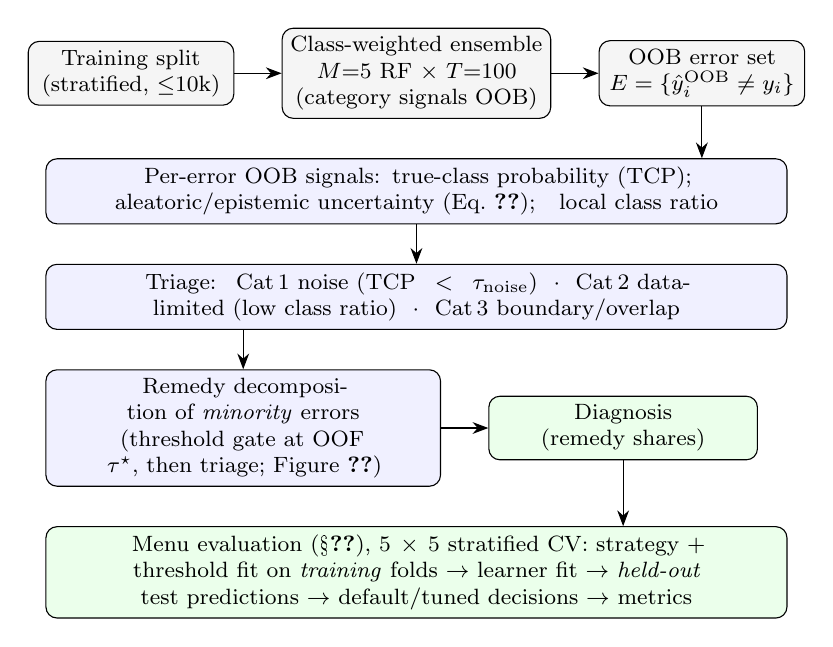
\begin{tikzpicture}[
  font=\footnotesize,
  stage/.style={draw, rounded corners, align=center, inner sep=3pt,
                minimum height=8mm, fill=black!4},
  sig/.style={stage, fill=blue!6},
  result/.style={stage, fill=green!8},
  >={Stealth[length=2mm]}, node distance=5mm and 6mm
]
\node[stage, text width=24mm] (data) {Training split\\(stratified, $\le$10k)};
\node[stage, right=of data, text width=32mm] (ens)
  {Class-weighted ensemble\\$M{=}5$ RF $\times$ $T{=}100$\\(category signals OOB)};
\node[stage, right=of ens, text width=24mm] (err)
  {OOB error set\\$E=\{\hat{y}^{\mathrm{OOB}}_i \ne y_i\}$};
\node[sig, below=of ens, text width=92mm] (sigs)
  {Per-error OOB signals: true-class probability (TCP);\quad
   aleatoric/epistemic uncertainty (Eq.~\ref{eq:uncertainty});\quad
   local class ratio};
\node[sig, below=of sigs, text width=92mm] (triage)
  {Triage: \ Cat\,1 noise ($\mathrm{TCP}<\tau_{\text{noise}}$) \ $\cdot$ \
   Cat\,2 data-limited (low class ratio) \ $\cdot$ \
   Cat\,3 boundary/overlap};
\node[sig, below=of triage, xshift=-22mm, text width=48mm] (remedy)
  {Remedy decomposition of \emph{minority} errors\\
   (threshold gate at OOF $\tau^\star$, then triage; Figure~\ref{fig:remedy})};
\node[result, right=of remedy, text width=32mm] (outp)
  {Diagnosis\\(remedy shares)};
\node[result, below=of remedy, xshift=22mm, text width=92mm] (eval)
  {Menu evaluation (\S\ref{sec:design}), $5\times5$ stratified CV: strategy +
   threshold fit on \emph{training} folds $\to$ learner fit $\to$ \emph{held-out}
   test predictions $\to$ default/tuned decisions $\to$ metrics};
\draw[->] (data) -- (ens);
\draw[->] (ens) -- (err);
\draw[->] (err.south) -- (err.south |- sigs.north);
\draw[->] (sigs) -- (triage);
\draw[->] (triage.south -| remedy.north) -- (remedy.north);
\draw[->] (remedy) -- (outp);
\draw[->] (outp.south) -- (outp.south |- eval.north);
\end{tikzpicture}
\caption{End-to-end pipeline. Every signal that drives the categorization (error
set, true-class probability, noise consensus) comes from out-of-bag predictions
of a class-weighted random-forest ensemble (the uncertainty values of
Eq.~\eqref{eq:uncertainty} interpret the categories and are recomputed fully
held-out in \appref{app:oof}); errors are triaged into three categories;
the misclassified minority is mapped to remedies via the threshold-recoverability
gate of \S\ref{sec:method:remedy}. The diagnosis is then evaluated against the
16-strategy menu under the protocol of \S\ref{sec:design}: $5\times5$ stratified
cross-validation in which each strategy (resampling, weighting, or
threshold-moving) and any tuned threshold are fit on the training folds only,
and all reported metrics come from the held-out test folds.}
\label{fig:pipeline}
\end{figure}

\subsection{Uncertainty decomposition via random forest ensembles}\label{sec:method:uncert}

We train an ensemble of $M=5$ random forests \cite{breiman2001random}, each with
$T=100$ trees and minimum leaf size $5$, on the full training set. For each
instance $\mathbf{x}_i$, each tree $t$ in forest $m$ produces a class probability
vector $\hat{p}_{m,t}(\mathbf{x}_i)$. Following Shaker and H\"ullermeier
\cite{shaker2020aleatoric,hullermeier2021aleatoric}, we decompose the total
predictive uncertainty:
\begin{equation}
\underbrace{H[\bar{p}(\mathbf{x}_i)]}_{\text{total}}
= \underbrace{\frac{1}{MT}\sum_{m,t} H[\hat{p}_{m,t}(\mathbf{x}_i)]}_{\text{aleatoric}}
+ \underbrace{H[\bar{p}(\mathbf{x}_i)] - \frac{1}{MT}\sum_{m,t} H[\hat{p}_{m,t}(\mathbf{x}_i)]}_{\text{epistemic}}
\label{eq:uncertainty}
\end{equation}
where $\bar{p}(\mathbf{x}_i) = \frac{1}{MT}\sum_{m,t}\hat{p}_{m,t}(\mathbf{x}_i)$
is the ensemble-averaged prediction and $H[\cdot]$ denotes Shannon entropy.
The ensemble size follows standard deep-ensemble practice ($M{=}5$,
\cite{lakshminarayanan2017simple}); a sensitivity analysis over
$M \in \{1,2,5,10,20\}$ shows the resulting categorization and remedy shares
are stable for $M \ge 5$ (category fractions move $\le 2.6$\,pp between $M{=}5$
and $M{=}20$; \appref{app:msens}), and \appref{app:nontree}
re-derives the full decomposition with bagged non-tree ensembles (MLPs,
logistic regression), with the headline unchanged.

The decomposition separates two distinct sources of error. Aleatoric uncertainty
captures the irreducibility of the data-generating process: it is high in regions
of genuine class overlap. Epistemic uncertainty captures the limits of the current
sample: it is high where the model has seen insufficient training data. This
distinction matters for rebalancing. Boundary-overlap errors (high aleatoric) are
not correctable by adding more data of the existing class; sparse-region errors
(high epistemic) are exactly where additional same-class evidence helps.

By contrast, the k-nearest-neighbour categorizations of Napiera{\l}a \&
Stefanowski \cite{napierala2016types} and related work \cite{smith2014instance}
measure only local same-class geometry, which conflates these two sources: an
instance with $0$ same-class neighbours might be a labelling error, a
Bayes-boundary point in a high-overlap region, or a genuinely under-represented
sparse instance. We use the aleatoric--epistemic decomposition purely as a
\emph{diagnostic} (to localize the boundary/overlap region on real data and
characterize the error population, \S\ref{sec:results}), not as a new
oversampler.

\paragraph{Out-of-bag estimation (no in-sample optimism).} Every
\emph{model-derived} signal that drives the categorization is computed from
\emph{out-of-bag} (OOB) predictions, i.e.\ for each instance, only from the
trees that did not bootstrap it. An instance is an \emph{error} if the OOB
ensemble majority vote disagrees with its label; the true-class probability (TCP,
\S\ref{sec:method:triage}) is the OOB estimate; the noise signals use OOB
confidence and consensus. The remaining signals (the local class ratio) are
properties of the data geometry, not model predictions. The error set and its
categories are therefore \emph{not} in-sample artefacts of forests fit and scored
on the same data. One quantity is scoped differently: the aleatoric/epistemic
values of Eq.~\eqref{eq:uncertainty} are computed over all trees of the fitted
instrument (in-bag included); they do not enter the category rules of
\S\ref{sec:method:triage}, serving as interpretation and validation, and the
strict check below recomputes them fully held-out. As a strict check we additionally re-derive the categories under
inner cross-validation (forests fit on inner-training folds categorize held-out
instances, so even the aleatoric/epistemic decomposition is out-of-fold); the
category distribution and the aleatoric/epistemic separation are essentially
unchanged (\appref{app:oof}). We then categorize each error instance.

\subsection{Three-way error categorization}\label{sec:method:triage}

For each error instance $\mathbf{x}_i$ we compute a \emph{local class ratio}: the
fraction of $k$-nearest neighbours sharing its label, normalized by the global
class frequency. Low values indicate the class is locally under-represented (a
data gap); high values indicate adequate local representation despite the error
(genuine overlap). The categorization rules are:
\begin{description}
\item[\textbf{Cat\,1 (Noise):}] $\mathrm{TCP}(\mathbf{x}_i) < \tau_{\text{noise}}$,
  where TCP is the ensemble true-class probability. Very low TCP indicates likely
  mislabeling; $\tau_{\text{noise}}=0.12$ gates noise from sparse-boundary errors.
\item[\textbf{Cat\,2 (Data-limited):}] not Cat\,1, and
  $\mathrm{class\_ratio}(\mathbf{x}_i) < \tau_{\text{cat2}}$ ($\tau_{\text{cat2}}=0.4$).
  The class is locally under-represented; the error arises from insufficient
  same-class data, not overlap.
\item[\textbf{Cat\,3 (Irreducible):}] neither Cat\,1 nor Cat\,2. The class is
  adequately represented locally yet the model errs, indicating genuine class
  overlap in a model-estimated Bayes-boundary/overlap region. (We reserve the term
  ``Bayes boundary'' for the controlled experiments of \S\ref{sec:results:mechanism}
  where it is known; on real data Cat\,3 is an \emph{estimate} of that region.)
\end{description}
The rules are deliberately operational --- ensemble confidence (TCP) and local
representation --- rather than thresholds on the uncertainty values of
Eq.~\eqref{eq:uncertainty} themselves; the aleatoric--epistemic decomposition
supplies the \emph{interpretation} of the resulting categories, and the held-out
validation confirms it (Cat\,3 aleatoric uncertainty exceeds Cat\,2's on $80\%$
of datasets, \appref{app:oof}).

To remove the imbalance bias of an off-the-shelf ensemble (a majority-biased
ensemble suppresses minority TCP and over-flags minority instances as noise), the
triage ensemble is trained with class-balanced instance weights (inverse class
frequency). Forest probability estimates respond only weakly to such weights
(\S\ref{sec:results:frontier}), and the \emph{unweighted} bagged instruments of
\appref{app:nontree} reproduce the decomposition, so the headline does not hinge
on this choice.

The two thresholds are fixed at $\tau_{\text{noise}}=0.12$, $\tau_{\text{cat2}}=0.4$
across \emph{all} datasets; they are defaults, not tuned hyperparameters. The
categorization is robust to their exact values: sweeping
$\tau_{\text{noise}}\in[0.05,0.30]$ and $\tau_{\text{cat2}}\in[0.2,0.6]$, $74\%$ of
datasets show $<0.5\%$ downstream-accuracy variation across all configurations, and
the category assignments preserve their relative structure throughout
(\appref{app:sensitivity}).

\subsection{Remedy decomposition of the minority deficit}\label{sec:method:remedy}

The triage characterizes \emph{why} an instance is hard; our central instrument
turns this into \emph{which remedy applies} to the instances that actually drive
the deficit --- the misclassified minority. Two instrument choices matter here
and we state them explicitly. First, the deficit being decomposed is that of the
\emph{default, off-the-shelf} model, so the decomposition is measured on the
\emph{unweighted} ensemble; the class-weighted variant of
\S\ref{sec:method:triage} partially enacts the operating-point shift inside the
instrument, leaving a harder residue, and is reported as a sensitivity
(\S\ref{sec:results:remedy}). Second, the error set is the ensemble's
\emph{actual} default prediction: a minority instance is a default error iff the
out-of-bag argmax over its mean probability vector differs from its label (on
binary tasks this coincides with $\Pr(\text{minority})<\tfrac12$; on multiclass
tasks the two differ, and the argmax definition is the valid one). For each such
error we ask, in order:
\begin{description}
\item[\textbf{Threshold-recoverable:}] is it classified \emph{correctly} under
  the decision-rule intervention that predicts the focal minority class whenever
  $\Pr(\text{minority})\ge\tau^\star$ and otherwise the highest-scoring remaining
  class (a one-vs-rest threshold move, valid for binary and multiclass alike),
  where $\tau^\star$ maximizes minority-vs-rest balanced accuracy? The threshold
  is \emph{cross-fitted}: instances are split into five stratified folds, and
  each instance's recovery is judged with a $\tau^\star$ selected on the other
  folds only, so no recovery decision uses a threshold chosen on that instance.
  If recovered, the model's score already places it on the minority side of the
  tuned operating point and only the default cutoff was wrong: the remedy is to
  change the decision rule, no data and no refitting required. This axis, which
  conditions on score-recoverability of an already-misclassified instance, is
  what distinguishes our decomposition from difficulty taxonomies.
\item[\textbf{Data-reducible (epistemic):}] otherwise, if the instance is Cat\,2
  (locally under-represented, high epistemic uncertainty), the remedy is more
  same-class data there (collection or targeted generation).
\item[\textbf{Irreducible (aleatoric):}] otherwise, if it is Cat\,3
  (model-estimated overlap, high aleatoric uncertainty), no remedy in our menu
  recovers it. On real data this is an \emph{estimated}-irreducible, aleatoric
  residue, not a proven Bayes-irreducible one.
\end{description}
(Cat\,1 noise is reported separately.) The $\Pr(\text{minority})$ scores used
here are out-of-bag with respect to model fitting, and $\tau^\star$ is
cross-fitted as above, so the decomposition is held out from both model fitting
and threshold selection (\appref{app:oof}). This three-way, remedy-mapped split
of the \emph{minority error population} is the paper's headline diagnostic; its
empirical shape (\S\ref{sec:results:remedy}) explains why a threshold move recovers
most of the deficit and identifies the minority of cases where data genuinely helps.

\paragraph{Remedy-irreducible is not the Cat\,3 set.} The remedy decomposition is
not a relabelling of the triage, and the \emph{irreducible} remedy class is much
smaller than the Cat\,3 (boundary/overlap) category (Figure~\ref{fig:remedy}). Two
things separate them.
First, the remedy decomposition runs only on the \emph{misclassified minority},
whereas the Cat\,3 fraction is reported over \emph{all} errors. Second, and more
importantly, it gives threshold-recoverability \emph{priority} over the triage
category: an error the triage places in the boundary/overlap region (Cat\,3) is
still counted \emph{threshold-recoverable} whenever the model ranks it above
$\tau^\star$: the default $\tfrac12$ cutoff was wrong, but the \emph{ranking} is
right. The irreducible remedy class therefore contains only the Cat\,3 minority
errors that remain misclassified \emph{after} the threshold move, a strict subset
of Cat\,3. This is why the irreducible remedy fraction ($\sim$17\% of the minority
deficit, \S\ref{sec:results:remedy}) is far below the Cat\,3 share of all errors
($\sim$85\%, \S\ref{sec:results:interventional}): most boundary errors are scored
well enough to be recovered by moving the decision, not by adding or accepting data.

\begin{figure}[t]
\centering
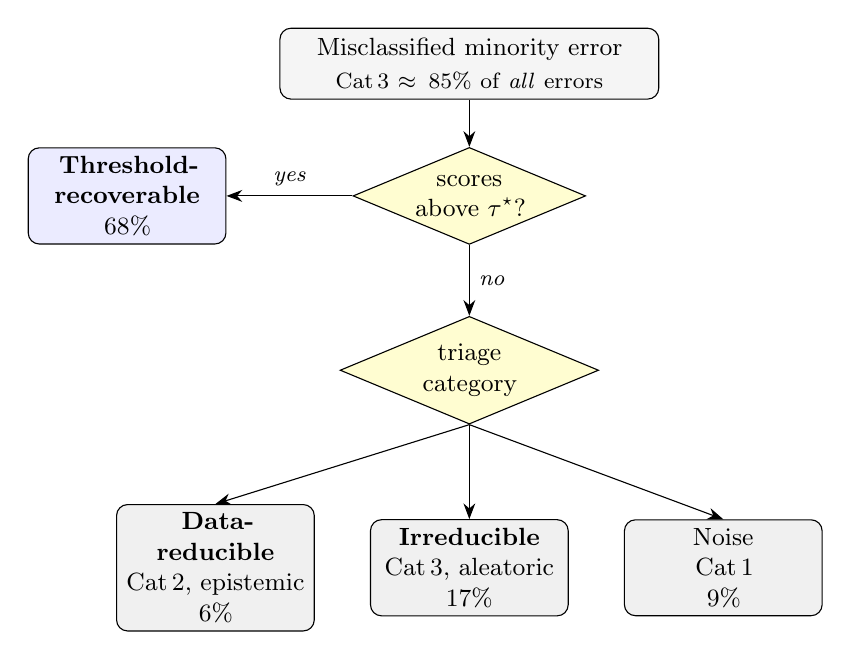
\begin{tikzpicture}[
  font=\small,
  box/.style={draw, rounded corners, align=center, inner sep=3pt, text width=23mm, minimum height=9mm},
  rem/.style={box, fill=blue!8},
  cat/.style={box, fill=black!6},
  q/.style={draw, diamond, aspect=2.4, align=center, inner sep=0pt, text width=17mm, fill=yellow!18},
  lbl/.style={font=\footnotesize\itshape},
  >={Stealth[length=2mm]}
]
\node[box, fill=black!4, text width=46mm] (err)
  {Misclassified minority error\\[1pt]{\footnotesize Cat\,3 $\approx 85\%$ of \emph{all} errors}};
\node[q, below=6mm of err] (q1) {scores above $\tau^\star$?};
\node[rem, left=16mm of q1] (tr) {\textbf{Threshold-}\\\textbf{recoverable}\\$68\%$};
\node[q, below=9mm of q1] (q2) {triage\\category};
\node[cat, below=12mm of q2] (c3) {\textbf{Irreducible}\\Cat\,3, aleatoric\\$17\%$};
\node[cat, left=7mm of c3] (c2) {\textbf{Data-reducible}\\Cat\,2, epistemic\\$6\%$};
\node[cat, right=7mm of c3] (c1) {Noise\\Cat\,1\\$9\%$};
\draw[->] (err) -- (q1);
\draw[->] (q1) -- node[above,lbl]{yes} (tr);
\draw[->] (q1) -- node[right,lbl]{no} (q2);
\draw[->] (q2.south) -- (c3.north);
\draw[->] (q2.south) -- (c2.north);
\draw[->] (q2.south) -- (c1.north);
\end{tikzpicture}
\caption{How the misclassified minority filters into the three remedy classes. The
decomposition asks threshold-recoverability \emph{first}: an error the model already
scores above the cross-fitted threshold $\tau^\star$ is \emph{threshold-recoverable}
whatever its triage category. Only the residue is split by triage into data-reducible
(Cat\,2), irreducible (Cat\,3), or noise (Cat\,1). Because most boundary (Cat\,3)
errors are well-scored, the \emph{irreducible} remedy class ($17\%$) is a strict
subset of Cat\,3 (which is itself $\sim$85\% of \emph{all} errors, \S\ref{sec:results:interventional}), which is why
$17\% \ll 85\%$. Percentages are means over datasets (Table~\ref{tab:reducibility}).}
\label{fig:remedy}
\end{figure}

\begin{table}[t]
\centering
\caption{The triage and remedy-decomposition procedure in pseudocode. All
model-derived quantities are out-of-bag (OOB) or out-of-fold (OOF); nothing is
fit and scored on the same data.}
\label{tab:algorithm}
\footnotesize
\begin{tabular}{@{}rp{0.86\linewidth}@{}}
\toprule
\multicolumn{2}{@{}l}{\textbf{Input:} training split $\mathcal{D}=\{(\mathbf{x}_i,y_i)\}$;
  $\tau_{\text{noise}}{=}0.12$, $\tau_{\text{cat2}}{=}0.4$; $M{=}5$, $T{=}100$, $k$} \\
\multicolumn{2}{@{}l}{\textbf{Output:} triage categories; remedy shares of the minority deficit} \\
\midrule
1 & Fit $M$ random forests ($T$ trees each, class-balanced instance weights); for each
    $\mathbf{x}_i$ collect the OOB tree probabilities $\hat{p}_{m,t}(\mathbf{x}_i)$
    and their mean $\bar{p}(\mathbf{x}_i)$. \\
2 & Error set $E \leftarrow \{i : \text{OOB majority vote} \ne y_i\}$. \\
3 & For each $i \in E$: $\mathrm{TCP}_i \leftarrow \bar{p}(\mathbf{x}_i)[y_i]$;
    aleatoric/epistemic uncertainty via Eq.~(\ref{eq:uncertainty});
    local class ratio $r_i \leftarrow$ fraction of $k$-nearest neighbours sharing
    $y_i$, normalized by the global frequency of $y_i$. \\
4 & \textbf{Triage:} Cat\,1 (noise) if $\mathrm{TCP}_i < \tau_{\text{noise}}$;
    else Cat\,2 (data-limited) if $r_i < \tau_{\text{cat2}}$;
    else Cat\,3 (boundary/overlap). \\
5 & \textbf{Threshold:} $\tau^\star \leftarrow \arg\max_{\tau}$ balanced accuracy
    of the rule $\bar{p}(\text{minority}\mid\mathbf{x}) \ge \tau$ on OOF
    predictions of the training split. \\
6 & \textbf{Remedy decomposition:} for each \emph{minority} $i \in E$:
    \emph{threshold-recoverable} if
    $\bar{p}(\text{minority}\mid\mathbf{x}_i) \ge \tau^\star$;
    else \emph{data-reducible} if Cat\,2; \emph{irreducible} if Cat\,3;
    \emph{noise} if Cat\,1. \\
7 & Return category fractions over $E$ and remedy shares over the minority errors. \\
\bottomrule
\end{tabular}
\end{table}

\subsection{Why boundary interpolation crosses the posterior boundary}\label{sec:method:theory}

The mechanism has a simple analytic basis. Let class~$1$ be the minority, write the
class-posterior $\eta(\mathbf{x})=\Pr(y{=}1\mid\mathbf{x})$, and let the Bayes
boundary be $\mathcal{B}=\{\mathbf{x}:\eta(\mathbf{x})=\tfrac12\}$ with
majority-posterior region $\mathcal{M}=\{\eta<\tfrac12\}$ (where the Bayes-optimal
label is the majority). SMOTE forms a synthetic point
$\mathbf{z}=\mathbf{x}_i+\lambda(\mathbf{x}_j-\mathbf{x}_i)$ with
$\lambda\sim\mathcal{U}(0,1)$, $\mathbf{x}_i$ a minority seed and $\mathbf{x}_j$
one of its minority $k$-nearest neighbours, and labels $\mathbf{z}$ as
\emph{minority}.

\begin{proposition}\label{prop:cross}
Assume $\eta$ is continuous along the segment $[\mathbf{x}_i,\mathbf{x}_j]$.
\begin{enumerate}
\item[(i)] Suppose a minority seed lies in the overlap region,
  $\eta(\mathbf{x}_i)<\tfrac12$, and is interpolated with a neighbour
  $\eta(\mathbf{x}_j)<\tfrac12$. By continuity $\mathcal{M}$ contains an
  $\varepsilon$-neighbourhood of each endpoint, so every \emph{sufficiently short}
  interpolation step from either endpoint yields $\mathbf{z}\in\mathcal{M}$; if in
  addition $\eta$ is quasiconvex along the segment (in particular, approximately
  affine, as in (ii)), then \emph{every} $\mathbf{z}\in[\mathbf{x}_i,\mathbf{x}_j]$
  lies in $\mathcal{M}$. Such a $\mathbf{z}$ carries a minority label in a region
  the Bayes rule assigns to the majority, i.e.\ it acts as label noise.
\item[(ii)] If the segment crosses $\mathcal{B}$, the probability that
  $\mathbf{z}\in\mathcal{M}$ equals
  $\big|\{\lambda\in[0,1]:\eta(\mathbf{x}_i+\lambda(\mathbf{x}_j-\mathbf{x}_i))<\tfrac12\}\big|\in(0,1)$.
  When $\eta$ is approximately affine over the segment with
  $\eta(\mathbf{x}_i)\ge\tfrac12>\eta(\mathbf{x}_j)$, this probability is
  $\dfrac{\tfrac12-\eta(\mathbf{x}_j)}{\eta(\mathbf{x}_i)-\eta(\mathbf{x}_j)}$.
\item[(iii)] Consequently the expected fraction of synthetic minority mass placed
  in $\mathcal{M}$ is non-decreasing in the local overlap (the minority probability
  mass near and beyond $\mathcal{B}$) and in the proportion of seeds drawn from the
  boundary/overlap region.
\end{enumerate}
\end{proposition}

\noindent\emph{Proof sketch.} (i) $\mathcal{M}=\{\eta<\tfrac12\}$ is the open
sublevel set of a continuous function, so it contains an $\varepsilon$-ball around
each interior endpoint and sufficiently short interpolation steps stay in
$\mathcal{M}$. A sublevel set need not be convex, so the segment is guaranteed to
remain in $\mathcal{M}$ \emph{in its entirety} only under the added quasiconvexity
(or approximately-affine) hypothesis; absent it, an interior excursion above
$\tfrac12$ is possible but does not affect the label-noise conclusion for the
points that do fall in $\mathcal{M}$. (ii) follows from the
intermediate value theorem and, in the affine case, from solving
$\eta(\mathbf{x}_i)+\lambda[\eta(\mathbf{x}_j)-\eta(\mathbf{x}_i)]=\tfrac12$ for the
crossing $\lambda^\star$ and integrating the uniform density over
$\{\eta<\tfrac12\}$. (iii) follows by taking expectations over the seed/neighbour
sampling distribution, whose support shifts toward $\mathcal{B}$ as overlap and
boundary-seed proportion grow. \hfill$\square$

This explains three observations below: standard SMOTE places an
\emph{overlap-dependent} fraction of synthetic points across a \emph{known}
boundary (\S\ref{sec:results:mechanism}); augmenting estimated-boundary (Cat\,3)
seeds reproduces the tradeoff while non-boundary seeds do not
(\S\ref{sec:results:interventional}); and boundary-\emph{targeting} variants
(Borderline-SMOTE, ADASYN) raise exactly the boundary-seed proportion of
clause~(iii), so they do not resolve the tradeoff.

\subsection{Strategy menu}\label{sec:method:menu}

We evaluate a menu of 16 rebalancing strategies grouped into five families:
(i)~\emph{do nothing}: train on the raw data;
(ii)~\emph{threshold-moving}: choose the decision threshold on out-of-fold
training predictions to maximize balanced accuracy (binary tasks), leaving the
data untouched;
(iii)~\emph{cost-sensitive}: class-balanced sample weights
\cite{elkan2001foundations}, and triage-informed weighting (upweighting the
correct same-class neighbours of Cat\,2 errors);
(iv)~\emph{generative oversampling}: SMOTE \cite{chawla2002smote} and eight
variants (Borderline-SMOTE, ADASYN, Safe-Level-SMOTE, ProWSyn, MWMOTE,
polynom-fit, Napierala-guided), plus \emph{clean-masked SMOTE} (SMOTE seeded only
from non-boundary, non-noise minority instances, i.e.\ excluding Cat\,1/Cat\,3);
at review we additionally evaluate the modern geometric variant G-SMOTE
\cite{douzas2019geometric} under the same protocol, reported alongside the
pre-registered menu rather than inside it
(\S\ref{sec:results:mechanism}, \S\ref{sec:results:frontier}, \appref{app:oversamplers});
(v)~\emph{balanced ensembles}: balanced random forest \cite{chen2004using} and
EasyEnsemble \cite{liu2009exploratory}.
The two triage-derived members (clean-masked SMOTE, triage weighting)
operationalize the diagnostic; as \S\ref{sec:results} shows they do not beat
the strong non-generative families, and we include them for completeness rather
than as headline methods.

\subsection{Meta-features and prescriptive selection}\label{sec:method:selection}

To ask whether a dataset's structure determines its best strategy, we describe
each dataset by meta-features in three groups: (a)~\emph{error-structure} from the
triage (Cat\,1/2/3 fractions and masses, minority error rate, learnable-minority
fraction); (b)~\emph{complexity / separability}: Fisher's maximum discriminant
ratio (F1) and the boundary/overlap measures N1, N2, N3 \cite{komorniczak2022data};
and (c)~\emph{basic} descriptors (imbalance ratio, size, dimensionality, class
count). A leave-one-dataset-out selector predicts, from these meta-features, which
menu strategy maximizes the target metric on the held-out dataset. We evaluate two
designs: a per-method regressor (predict each strategy's score, take the
argmax) and a direct method-classifier. We compare both against fixed baselines (always-SMOTE,
the best single fixed strategy), an imbalance-ratio-only rule, and a per-dataset
oracle. Significance is assessed by paired Wilcoxon tests across datasets with
bootstrap confidence intervals, and selector stability is checked across random
seeds.

\section{Experimental Design}\label{sec:design}

\paragraph{Datasets.} We evaluate on 79 real classification datasets: the 27
datasets of the \texttt{imbalanced-learn}/KEEL benchmark suite (imbalance ratios
$8$--$130$) and 52 of the 54 OpenML \cite{vanschoren2014openml} and scikit-learn
datasets listed in \appref{app:datasets} (USPS and webpage are excluded from
the menu evaluation for high dimensionality and sparse formatting), spanning binary
and multiclass problems with original sizes from $150$ to $581{,}012$ instances and
$4$ to $500$ features. We apply stratified
subsampling to a maximum of $10{,}000$ instances per dataset, which preserves the
triage category distribution (mean absolute deviation $<2$\,pp per category,
\appref{app:subsampling}). The interventional experiment
(\S\ref{sec:results:interventional}) uses the 50 datasets where minority
size permits SMOTE seed-pool slicing. The OpenML roster is listed in
\appref{app:datasets}.

\paragraph{Strategy menu and base learner.} We evaluate the 16-strategy menu of
\S\ref{sec:method:menu}. The base learner for non-ensemble strategies is
XGBoost \cite{chen2016xgboost} (300 trees, max depth 6, learning rate 0.1);
balanced random forest (300 trees) and EasyEnsemble (10 AdaBoost members) are
themselves ensemble learners. We use $5\times5$ Repeated Stratified $K$-Fold
cross-validation; the triage and the moved threshold are fit on the training
split only (threshold chosen on out-of-fold training predictions, so there is no
test leakage). Binary-only strategies (threshold-moving, EasyEnsemble) are skipped
on multiclass datasets and excluded from those datasets' candidate sets.

\paragraph{Metrics.} Balanced accuracy is the primary metric --- it is the
objective that motivates rebalancing --- and we report accuracy alongside it to
expose the tradeoff, plus G-mean and MCC as tradeoff-internalizing checks. We
report win rates and Wilcoxon signed-rank \cite{wilcoxon1945individual}
$p$-values; per-dataset values are means over the $25$ folds.

\paragraph{Selection protocol.} The prescriptive selector
(\S\ref{sec:method:selection}) is evaluated leave-one-dataset-out across the
79 datasets: for each held-out dataset the selector is trained on the other 78 and
its chosen strategy's realized metric is recorded. We compare against a per-dataset
oracle, the best single fixed strategy, always-SMOTE, an imbalance-ratio-only rule,
and random choice, with paired Wilcoxon tests, bootstrap confidence intervals on
the mean gain, and a seed-robustness check over 8 random seeds.

\paragraph{Pre-registration.} To avoid post-hoc selection of the analysis, we
pre-specified the primary selector (a per-method regressor over all meta-features)
and the primary metric (balanced accuracy) before running the full-menu
evaluation. The direct method-classifier and the parsimonious feature set are
reported as secondary analyses, and we disclose in full that the pre-registered
regressor only ties the best fixed strategy while the classifier modestly beats it
(\S\ref{sec:results:selection}).

\section{Results}\label{sec:results}

We proceed from validating the triage, to the headline remedy decomposition (the
deficit is mostly threshold-recoverable), to the mechanism (controlled overlap and
a proposition), to its consequence at scale (oversampling is an operating-point
move: no ranking gain, worse calibration, and a tie with threshold-moving at
parity), and finally to the prescription (a regime map and an honestly-scoped
selector).

\subsection{Error Instance Triage: validation}\label{sec:results:validation}

\paragraph{Synthetic ground truth.} On two-class Gaussian mixtures the triage
behaves as designed. As class separation shrinks from $1.2$ to $0.2$ standard
deviations (overlap grows), the Cat\,3 (irreducible) fraction among errors rises
monotonically, exceeding $95\%$ at the smallest separation (mean $94.3\%$ across
the sweep) --- the triage correctly attributes boundary-overlap errors to
irreducibility. On 24 real datasets with $5\%$ injected label noise the triage
detects the flips with mean precision $0.77$, and the flagged-noise fraction rises
significantly ($p=2\times10^{-5}$, Wilcoxon). The triage is thus sensitive to both
boundary overlap (Cat\,3) and label noise (Cat\,1), the two categories that drive
the mechanism below.

\paragraph{Out-of-fold robustness.} Because the categories underpin the mechanistic
argument, we verify they are not in-sample artefacts. The category assignment
already uses out-of-bag predictions (\S\ref{sec:method:uncert}); under a strict
inner cross-validation that re-derives \emph{every} signal --- including the
aleatoric/epistemic decomposition --- on held-out instances, the Cat\,3 fraction
among errors is essentially unchanged (in-sample $\to$ out-of-fold mean shift of
$\approx\!\OOFCATSHIFT$\,pp over 79 datasets) and the aleatoric/epistemic ordering
that defines the categories is preserved (\appref{app:oof}).

\paragraph{Is the triage a uniquely good predictor of SMOTE harm? No --- and it
need not be.} A reviewer will rightly ask whether the aleatoric--epistemic triage
is necessary or whether a simpler $k$-NN hardness / overlap score localizes
SMOTE's harm equally well. Across the 75 datasets with a SMOTE outcome we correlate
eleven per-dataset measures with SMOTE's accuracy cost (Table~\ref{tab:ablation}).
The trivial \emph{minority error rate} is the strongest single predictor
($\rho=-0.49$, leave-one-out $R^2=0.34$), with the Napiera{\l}a rare/outlier
fraction and the imbalance ratio close behind ($\rho\approx-0.40$); the triage's
Cat\,3 mass is only a moderate, marginally significant predictor ($\rho=-0.21$,
$p=0.07$). The \emph{conditional} Cat\,3 fraction (\texttt{frac\_cat3}) even
correlates with \emph{less} accuracy harm ($\rho=+0.37$): the fraction of errors
that are boundary errors is not the dataset-level \emph{mass} of boundary-entangled
minority, and a dataset can carry a high Cat\,3 share within a \emph{small} error
population --- a near-ceiling problem SMOTE barely perturbs. The mechanism is tied
to that boundary mass (better captured by the minority error rate), not the
conditional fraction alone. We state this plainly: the triage is \emph{not} a better
cross-dataset forecaster of SMOTE harm than simple measures, and we do not claim it
is. Its role
is \emph{explanatory} --- it localizes \emph{which} errors lie in the
boundary/overlap region so the intervention of
\S\ref{sec:results:interventional} can seed augmentation there and probe the
mechanism --- not a predictive instrument, consistent with the honest selection
finding of \S\ref{sec:results:selection}. Put differently, the minority error rate
predicts the \emph{size} of the deficit; the remedy decomposition diagnoses the
\emph{appropriate intervention}.

\begin{table}[t]
\centering
\caption{Triage-design ablation: Spearman correlation of each per-dataset measure
with SMOTE's accuracy change ($\Delta$acc) and balanced-accuracy change
($\Delta$bacc), and a single-feature leave-one-out $R^2$ for $\Delta$acc, over 75
datasets. The triage's Cat\,3 mass is not a stronger predictor of SMOTE harm than
simple hardness/imbalance measures; the triage's value is explanatory, not
predictive. $^{*}$: $p<0.05$.}
\label{tab:ablation}
\begin{tabular}{lrrr}
\toprule
Per-dataset measure & $\rho$(SMOTE $\Delta$acc) & $\rho$($\Delta$bacc) & LOO $R^2$($\Delta$acc) \\
\midrule
minority error rate & -0.49$^{*}$ & +0.57 & 0.34 \\
Napierala rare+outlier & -0.40$^{*}$ & +0.58 & 0.17 \\
imbalance ratio & -0.40$^{*}$ & +0.76 & -0.23 \\
frac\_cat3 (triage) & +0.37$^{*}$ & -0.53 & -0.00 \\
LOO 1-NN error (N3) & -0.24$^{*}$ & -0.06 & -0.01 \\
cat3\_mass (triage) & -0.21 & -0.12 & -0.01 \\
boundary frac (N1) & -0.20 & -0.15 & -0.02 \\
Fisher F1 & -0.13 & +0.45 & 0.01 \\
instance hardness (max\_fdr) & +0.13 & -0.45 & -0.04 \\
intra/extra ratio (N2) & +0.06 & +0.34 & -0.03 \\
Napierala borderline & +0.02 & +0.04 & -0.03 \\
\bottomrule
\end{tabular}

\end{table}

\subsection{The minority deficit is mostly threshold-recoverable}\label{sec:results:remedy}

\paragraph{Result.} We apply the remedy decomposition (\S\ref{sec:method:remedy})
to the misclassified minority on every dataset (Table~\ref{tab:reducibility}).
Across the 70 datasets with a non-trivial minority error set, the deficit is
\textbf{predominantly threshold-recoverable}: a mean of $\mathbf{69\%}$ (median
$75\%$) of minority errors are corrected simply by moving the decision threshold to
its out-of-fold balanced-accuracy optimum --- the model already \emph{ranked} these
instances correctly. Only $7\%$ are data-reducible (epistemic --- where more
same-class data would help), $16\%$ are irreducible (aleatoric --- model-estimated
overlap), and $7\%$ are noise. The pattern \emph{sharpens} with imbalance: on
$\mathrm{IR}>3$ datasets $74\%$ of the deficit is threshold-recoverable. This is
corroborated independently by separability: on the 30 hardest binary datasets
(baseline balanced accuracy $<0.85$) the baseline classifier's out-of-fold AUC is a
median of $0.91$ ($93\%$ exceed $0.70$) --- the classes are well ranked even where
default-threshold balanced accuracy is poor. (The genuine exceptions, AUC
$\approx0.59$, are the near-irreducible problems.)

\paragraph{Consistency with Cat\,3 dominating the errors.} The $\sim$85\% Cat\,3
share reported below (\S\ref{sec:results:interventional}) and the $16\%$ irreducible
fraction here are not in tension (\S\ref{sec:method:remedy}). Cat\,3 is a triage
label for errors in the estimated overlap region under the \emph{default} decision
rule, computed over \emph{all} errors; the remedy decomposition then asks, for the
\emph{minority} errors only, whether that default-threshold mistake survives a move
to the tuned operating point $\tau^\star$. Because the classifier ranks most of
these boundary errors above $\tau^\star$, they are counted threshold-recoverable,
and only the residue the threshold move cannot rescue is counted irreducible --- a
strict subset of the minority Cat\,3 errors, not the whole category.

\begin{table}[t]
\centering
\caption{Remedy decomposition of the misclassified minority (mean over datasets,
out-of-bag): the fraction of minority errors that are threshold-recoverable (a
threshold move corrects them), data-reducible (epistemic; more minority data
helps), irreducible (aleatoric; model-estimated overlap), or noise. The deficit is
predominantly a thresholding artefact, increasingly so with imbalance.}
\label{tab:reducibility}
\begin{tabular}{lrrrr}
\toprule
Subset & threshold-recoverable & data-reducible & irreducible & noise \\
\midrule
All datasets & 68\% & 6\% & 17\% & 9\% \\
$\mathrm{IR}>3$ & 80\% & 4\% & 5\% & 12\% \\
$\mathrm{IR}>10$ & 80\% & 5\% & 2\% & 13\% \\
Binary & 69\% & 4\% & 15\% & 12\% \\
Multiclass & 67\% & 10\% & 22\% & 1\% \\
\bottomrule
\end{tabular}

\end{table}

\paragraph{Why this matters.} This decomposition is the mechanistic account of a
well-documented but unexplained regularity --- that resampling does not improve
ranking and a threshold move reproduces its benefit
\cite{provost2000imbalanced,elkan2001foundations,elor2022smote,goorbergh2022harm}.
\emph{Because} most of the minority deficit is threshold-recoverable, a
non-generative change of the decision rule recovers it, and oversampling --- which
leaves ranking unchanged (\S\ref{sec:results:frontier}) --- is at best an implicit,
inefficient way to enact the same threshold move. The decomposition also tells a
practitioner \emph{which} situation they are in: the (minority) data-reducible
fraction is where collecting or generating minority data is warranted; the
irreducible fraction is where no remedy in our evaluated menu helps.

\subsection{Mechanism: SMOTE generates across the Bayes boundary}\label{sec:results:mechanism}

\paragraph{Premise.} If SMOTE's accuracy cost arises from generation near the
Bayes boundary, then on a controlled problem with a \emph{known} boundary,
standard SMOTE should place synthetic minority points \emph{across} that boundary
--- in majority territory, where they act as label noise --- increasingly so as
overlap grows, while excluding the irreducible seeds should prevent it.

\paragraph{Result.} We generate 2D Gaussian classes
($\mathcal{N}([\pm s,0], I)$, $9{:}1$ imbalance, balanced Bayes boundary
$x=0$) and sweep the separation $s$. Standard SMOTE places an
\emph{overlap-dependent} fraction of its synthetic minority points on the
majority side of the boundary --- from $6\%$ at $s=1.5$ to $34\%$ at $s=0.4$ ---
whereas masking the Cat\,3 (boundary) seeds generates essentially none
($\le 2\%$, $0\%$ for $s\ge0.8$); Figure~\ref{fig:overlap} visualizes both.

\begin{figure}[t]
\centering
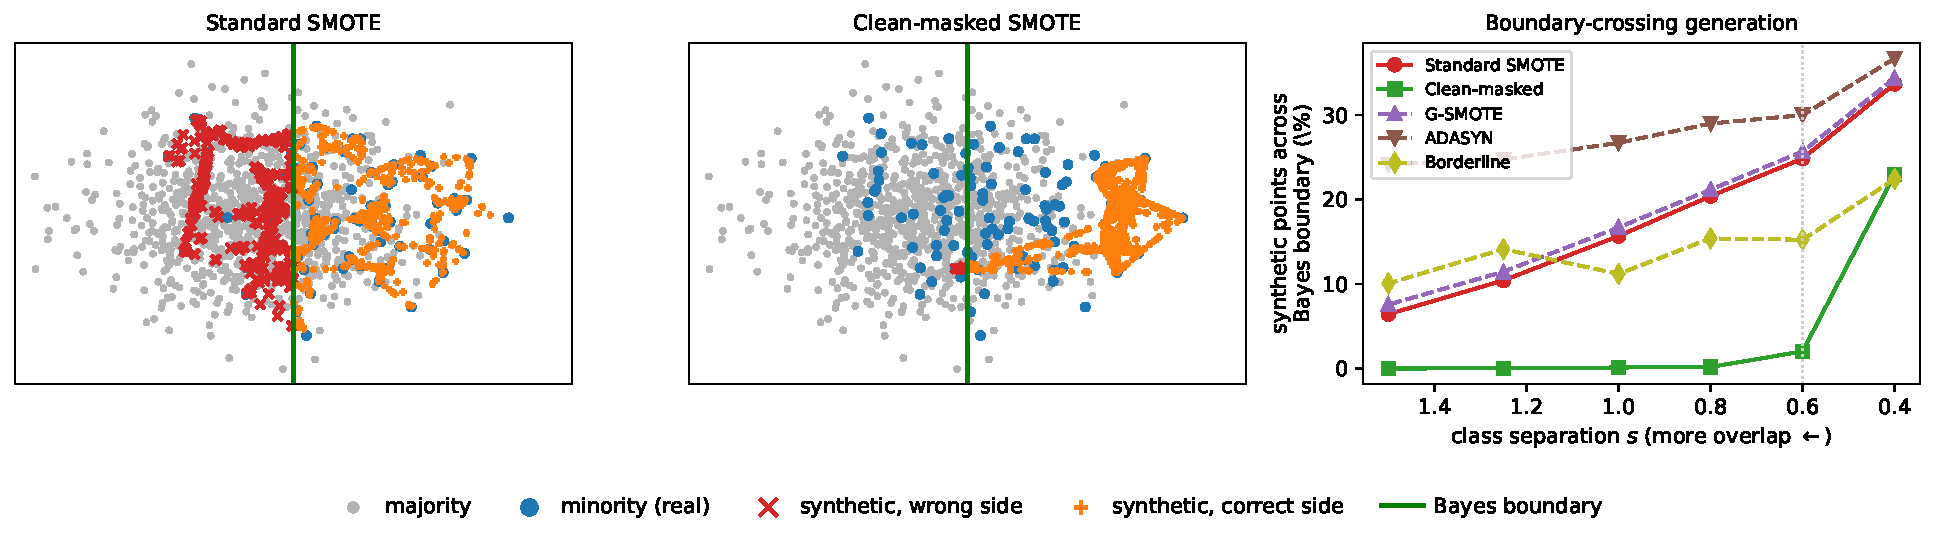
\includegraphics[width=\linewidth]{figures/fig_overlap.pdf}
\caption{Mechanism on controlled 2D Gaussians ($9{:}1$; balanced Bayes boundary
$x=0$, green). Left/middle: at moderate overlap ($s=0.6$) standard SMOTE scatters
synthetic minority points (red $\times$) across the boundary into majority
territory; masking the boundary seeds keeps generation on the minority side.
Right: the fraction of synthetic points crossing the boundary rises with overlap
for SMOTE but stays near zero when boundary seeds are excluded.}
\label{fig:overlap}
\end{figure}

\subsection{Interventional evidence}\label{sec:results:interventional}

\paragraph{Premise.} If the accuracy--balanced-accuracy tradeoff is \emph{caused}
by generation near the (estimated) boundary, then targeted generation around
Cat\,3 (irreducible) errors should reproduce the SMOTE signature, while
random-instance generation should not.

\paragraph{Protocol.} On each training fold we compute the triage and, for each
strategy, append a \emph{fixed} budget $B$ of synthetic points equal to the total
number of triage errors on that fold --- identical across strategies, so the
comparison isolates \emph{where} one generates, not how much. Synthetic points are
produced by SMOTE-style interpolation \emph{within the targeted seed subset only}
(each synthetic point takes its seed's own class, with $B$ split across classes in
proportion to the seed subset's class distribution); all original training instances
are kept, and the data are \emph{not} rebalanced to a fixed ratio. The six
strategies are: \texttt{augment\_cat2} and \texttt{augment\_cat3} (seeds from the
respective error category), \texttt{augment\_all\_errors} (all errors),
\texttt{augment\_random} (a size-$B$ random sample of \emph{all} training instances
--- class-proportional, hence a true null that cannot shift the class balance), and
two removal controls (\texttt{remove\_noise}, \texttt{remove\_random}). The base
learner is XGBoost; metrics are over $5\times5$ folds. Seeds come from the triage on
the training fold. This real-data intervention is a \emph{small} effect and, as we
report honestly, sensitive to seed re-estimation (\appref{app:oof}); we treat
it as corroboration of, not primary evidence for, the mechanism --- which rests on
the controlled experiment (\S\ref{sec:results:mechanism}, known boundary) and the
discrimination/threshold analysis (\S\ref{sec:results:frontier}).

\paragraph{Result.} We run these strategies on each of 50 datasets against a
no-augmentation baseline. Augmenting Cat\,3 errors
recreates the signature tradeoff: balanced accuracy improves (win rate $68\%$,
$p=0.001$) while accuracy trends negative. Augmenting all errors amplifies it
($p<0.001$) because Cat\,3 dominates the error population ($\sim$86\%). Crucially,
\emph{random} augmentation produces no effect on either metric (WR $\approx50\%$,
$p>0.5$), and augmenting Cat\,2 errors helps balanced accuracy modestly
($p=0.007$) without harming accuracy (Figure~\ref{fig:interventional}).

\begin{figure}[t]
\centering
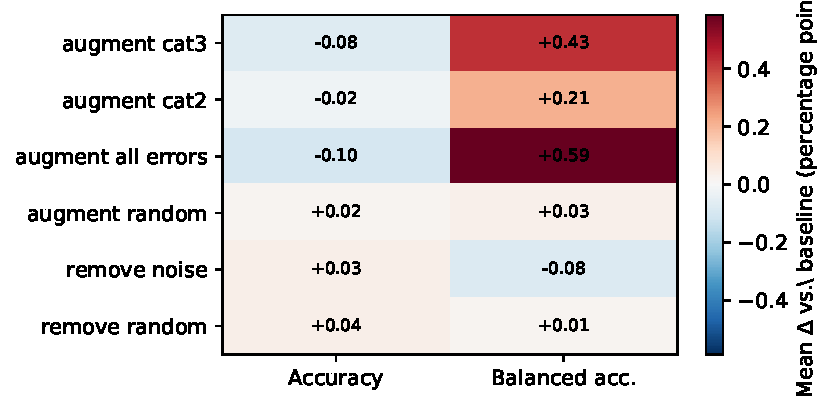
\includegraphics[width=\linewidth]{figures/fig1_interventional.pdf}
\caption{Interventional validation: mean metric change vs.\ the no-augmentation
baseline by augmentation target (50 datasets, fixed budget). Cat\,3
(boundary) augmentation reproduces the SMOTE signature --- balanced-accuracy gain
at an accuracy cost --- while random augmentation is null.}
\label{fig:interventional}
\end{figure}

\paragraph{Interpretation.} Consistent with the mechanism, the targeted-augmentation
contrast points to generation in the model-estimated boundary/overlap region
(Cat\,3) as the source of the accuracy cost, with the random-augmentation control
null. We are deliberately measured here: this is a \emph{small} real-data effect
that manipulates \emph{model-estimated} hard instances (not the true, unobserved
Bayes boundary), and it weakens under strict out-of-fold seed re-estimation at
reduced power (\appref{app:oof}). The mechanism does not rest on it: the
controlled experiment of \S\ref{sec:results:mechanism} (known boundary) and the
discrimination/threshold analysis of \S\ref{sec:results:frontier} (oversampling
does not improve ranking; its gain is a recoverable operating-point shift) are the
load-bearing evidence.

\subsection{Oversampling is an operating-point move, not a discrimination gain}\label{sec:results:frontier}

We now confirm the consequence the decomposition predicts, on the full menu and at
scale. The results in this section reproduce known findings
\cite{provost2000imbalanced,elor2022smote,goorbergh2022harm,dalpozzolo2015calibrating}
on a broad roster; we present them as confirmation that grounds the mechanism, not
as new claims.

\paragraph{No discrimination gain; worse calibration.} Oversampling does not help
the classifier \emph{rank}: on the binary datasets, SMOTE's out-of-fold ROC-AUC
($0.911$) and PR-AUC (at fixed test prevalence, $0.653$) are statistically
indistinguishable from the unresampled baseline ($0.909$, $0.655$), while its
probability calibration is worse (Brier $0.031$ vs.\ $0.028$; expected calibration
error $0.030$ vs.\ $0.025$), with Safe-Level-SMOTE worst (Table~\ref{tab:metrics}).
This matches the established account that resampling leaves ranking intact and
shifts only the threshold-dependent operating point, at a calibration cost
\cite{dalpozzolo2015calibrating,goorbergh2022harm,carriero2025harms}. Whatever
balanced-accuracy SMOTE buys is therefore an operating-point move, not a better
classifier.

\paragraph{At threshold parity, oversampling adds little.} The headline ``win''
of non-generative strategies is itself an operating-point artefact. At the
\emph{default} threshold, non-generative strategies top the balanced-accuracy
ranking on both rosters (best non-gen $\ge$ best gen on balanced accuracy in
$25/27$ KEEL datasets, $+5.76$\,pp, $95\%$ CI $[+3.81,+7.90]$; $43/52$ OpenML,
$+2.02$\,pp, $[+1.20,+2.98]$; $86\%$ overall; Friedman--Nemenyi
Figure~\ref{fig:cd}, $\chi^2{=}285.6$, $p<10^{-50}$, threshold-moving best rank
$3.15$) --- but only because threshold-moving is tuned and the SMOTE family is
scored at $0.5$. When \emph{every} strategy receives the same out-of-fold
threshold tuning, almost the entire gap disappears: on the 27 KEEL binary datasets
a tuned threshold alone lifts SMOTE's balanced accuracy by $+6.4$\,pp, and the
best-non-generative\,$-$\,best-generative difference collapses from $+5.76$\,pp at
the default threshold to within $\pm1$\,pp at parity (Table~\ref{tab:parity}:
$-0.72$\,pp for XGBoost, $-0.49$ for RF, $+0.19$ for logistic regression). We are
precise about the residual: at parity the best \emph{generative} strategy is in
fact marginally \emph{ahead} on XGBoost ($0.72$\,pp, $p{=}0.003$) and RF
($p{=}0.06$), and tied on logistic regression --- but this sub-$1$\,pp edge comes
with \emph{no} ranking gain and \emph{worse} calibration (above), against a
$+6.4$\,pp threshold effect. The decisive lever is therefore the \emph{threshold},
not the generative/non-generative choice, which is a fraction of its size. This
corroborates, on a 16-strategy menu and three learners, the broader-roster
conclusion of \cite{elor2022smote} (73 datasets) and \cite{goorbergh2022harm} that
balancing and threshold-tuning yield equivalent discrimination.

\begin{table}[t]
\centering
\caption{Probability metrics by strategy (XGBoost, mean over the 27 KEEL binary
datasets, out-of-fold). Oversampling does not improve ranking (ROC-AUC, PR-AUC at
fixed prevalence) and worsens calibration (Brier, expected calibration error);
recall at $10\%$ false-positive rate is likewise unimproved.}
\label{tab:metrics}
\small
\begin{tabular}{lrrrrrrr}
\toprule
 & none & cost & SMOTE & Border & ADASYN & SafeLvl & G-SMOTE \\
\midrule
ROC-AUC & 0.909 & 0.905 & 0.911 & 0.910 & 0.910 & 0.905 & 0.908 \\
PR-AUC & 0.655 & 0.652 & 0.653 & 0.650 & 0.649 & 0.632 & 0.649 \\
Brier & 0.028 & 0.034 & 0.031 & 0.031 & 0.032 & 0.040 & 0.031 \\
Brier (bal.) & 0.205 & 0.169 & 0.169 & 0.175 & 0.168 & 0.160 & 0.186 \\
ECE & 0.025 & 0.035 & 0.030 & 0.029 & 0.031 & 0.044 & 0.030 \\
ECE (bal.) & 0.233 & 0.182 & 0.185 & 0.192 & 0.185 & 0.170 & 0.209 \\
Rec@FPR10 & 0.775 & 0.766 & 0.774 & 0.775 & 0.773 & 0.751 & 0.773 \\
ROC-AUC rank & 4.02 & 4.94 & 3.65 & 3.76 & 3.65 & 4.74 & 3.24 \\
Brier rank & 2.63 & 3.93 & 3.85 & 4.04 & 4.59 & 6.00 & 2.96 \\
\bottomrule
\end{tabular}

\end{table}

\begin{table}[t]
\centering
\caption{Threshold parity: best non-generative $-$ best generative balanced
accuracy when \emph{every} strategy is given the same out-of-fold threshold tuning,
per base learner (27 KEEL binary datasets). The difference is within $\pm1$\,pp on
every learner (a small generative edge on XGBoost/RF, tied on logistic regression),
versus a $+5.76$\,pp non-generative advantage at the default threshold --- the
default-threshold ``dominance'' is overwhelmingly an operating-point effect.}
\label{tab:parity}
\begin{tabular}{lrrrr}
\toprule
Base learner & $n$ & NG$\ge$G & non-gen advantage & paired $p$ \\
\midrule
XGBoost & 27 & 19\% & $-0.72$ [-1.52,-0.18] & $0.003$ \\
Random forest & 26 & 27\% & $-0.49$ [-1.11,-0.03] & $0.06$ \\
Logistic regression & 27 & 59\% & $+0.19$ [-0.06,+0.43] & $0.2$ \\
\bottomrule
\end{tabular}

\end{table}

\paragraph{The default-threshold gap scales with imbalance.} Because the deficit
grows with imbalance, so does the (operating-point) penalty of leaving SMOTE at the
default threshold (Table~\ref{tab:irstrata}): the default-threshold non-generative
advantage rises from $+4.45$\,pp at $\mathrm{IR}>1.5$ to $+5.78$\,pp at
$\mathrm{IR}>10$, and SMOTE's accuracy cost deepens in lockstep ($-0.37 \to
-0.72$\,pp) as its balanced-accuracy gain grows ($+2.30 \to +4.28$\,pp). The
tradeoff is dose-responsive to imbalance, exactly as the boundary mechanism
predicts; the parity result above shows this default-threshold gap is recoverable
by a threshold move rather than by generation.

\paragraph{The cost tracks the mechanism.} SMOTE's per-dataset accuracy loss scales
with the minority error rate ($\rho=-0.50$, $p<10^{-4}$) and the imbalance ratio
($\rho=-0.41$, $p<10^{-3}$): it hurts most exactly where the minority is most
boundary-entangled and rebalancing is most aggressive --- the regime the mechanism
predicts.

\begin{table}[t]
\centering
\caption{The default-threshold non-generative advantage and the SMOTE tradeoff by
data stratum (existing benchmark cells, no re-run), all at the \emph{default}
threshold. NG$\ge$G is the fraction of datasets where the best non-generative
strategy matches/beats the best generative one on balanced accuracy; ``bacc adv.''
is the mean per-dataset advantage; the last two columns are SMOTE's mean accuracy
and balanced-accuracy change vs.\ the do-nothing baseline (percentage points). The
gap grows with imbalance but is an operating-point effect (Table~\ref{tab:parity}).}
\label{tab:irstrata}
\begin{tabular}{lrrrrr}
\toprule
Subset & $n$ & NG$\ge$G & bacc adv. & SMOTE $\Delta$acc & SMOTE $\Delta$bacc \\
\midrule
$\mathrm{IR}>1.5$ & 53 & 87\% & +4.45 & -0.56 & +3.20 \\
$\mathrm{IR}>3$ & 44 & 89\% & +5.27 & -0.61 & +3.72 \\
$\mathrm{IR}>10$ & 32 & 88\% & +5.78 & -0.72 & +4.28 \\
binary only & 46 & 85\% & +4.35 & -0.35 & +2.96 \\
multiclass only & 29 & 90\% & +1.86 & -0.39 & +1.24 \\
high-overlap & 26 & 77\% & +1.68 & -0.42 & +1.45 \\
\bottomrule
\end{tabular}

\end{table}

\paragraph{Not a base-learner artefact.} The pattern is not specific to
gradient-boosted trees. With random-forest and logistic-regression base learners
the default-threshold non-generative advantage persists ($+2.07$\,pp, $75\%$,
$p=1.6\times10^{-4}$ for RF; $+6.44$\,pp, $96\%$, $p=2\times10^{-10}$ for logistic
regression, the most miscalibrated learner) --- and the threshold-parity analysis
(Table~\ref{tab:parity}) likewise holds across all three learners, confirming the
gap is an operating-point effect rather than a property of any one model family.

\begin{table}[!tp]
\centering
\caption{Per-strategy mean accuracy / balanced accuracy across the 16-strategy
menu (XGBoost base learner; KEEL, $n{=}27$; OpenML, $n{=}52$), sorted by mean
balanced accuracy. \emph{At the default decision threshold}, non-generative
strategies ($\dagger$) occupy the top of the balanced-accuracy ranking on both
rosters and the entire SMOTE family sits below them, but this ranking gap is
largely an operating-point effect that collapses once every strategy receives the
same out-of-fold threshold tuning (Table~\ref{tab:parity}). Entries are means
over the $25$ folds; ``rank'' is the mean
per-dataset balanced-accuracy rank over the full menu on the $N{=}46$ binary
datasets (lower is better; the ranking of Figure~\ref{fig:cd}; the sixteenth
member, the balanced clean-masked variant, rank $9.88$, is not shown). The
significance of the default-threshold advantage (paired Wilcoxon $p<10^{-10}$,
bootstrap $95\%$ CIs) is reported in \S\ref{sec:results:frontier}.}
\label{tab:frontier}
\small
\begin{tabular}{l c cc cc c}
\toprule
 & & \multicolumn{2}{c}{KEEL} & \multicolumn{2}{c}{OpenML} & \\
\cmidrule(lr){3-4}\cmidrule(lr){5-6}
Strategy & type & acc & bacc & acc & bacc & rank \\
\midrule
threshold-moving        & $\dagger$ & 0.863 & \textbf{0.856} & 0.854 & \textbf{0.858} & \textbf{3.15} \\
balanced RF             & $\dagger$ & 0.910 & \textbf{0.855} & 0.812 & 0.812 & 5.05 \\
EasyEnsemble            & $\dagger$ & 0.847 & \textbf{0.854} & 0.815 & \textbf{0.822} & 6.39 \\
cost-sensitive          & $\dagger$ & 0.958 & 0.802 & 0.849 & 0.793 & 6.92 \\
SMOTE                   &           & 0.961 & 0.800 & 0.851 & 0.793 & 6.64 \\
Safe-Level-SMOTE        &           & 0.948 & 0.806 & 0.848 & 0.790 & 6.46 \\
ADASYN                  &           & 0.960 & 0.801 & 0.851 & 0.791 & 7.13 \\
Borderline-SMOTE        &           & 0.961 & 0.795 & 0.851 & 0.791 & 7.68 \\
ProWSyn                 &           & 0.961 & 0.800 & 0.853 & 0.787 & 7.14 \\
MWMOTE                  &           & 0.960 & 0.795 & 0.852 & 0.786 & 8.71 \\
Napierala-guided SMOTE  &           & 0.964 & 0.783 & 0.851 & 0.789 & 10.04 \\
clean-masked SMOTE      &           & 0.964 & 0.779 & 0.852 & 0.786 & 10.83 \\
polynom-fit SMOTE       &           & 0.966 & 0.766 & 0.854 & 0.780 & 12.78 \\
triage weighting        & $\dagger$ & 0.967 & 0.761 & 0.854 & 0.778 & 13.47 \\
baseline (do nothing)   & $\dagger$ & 0.967 & 0.761 & 0.854 & 0.777 & 13.72 \\
\bottomrule
\end{tabular}
\end{table}


\begin{figure}[t]
\centering
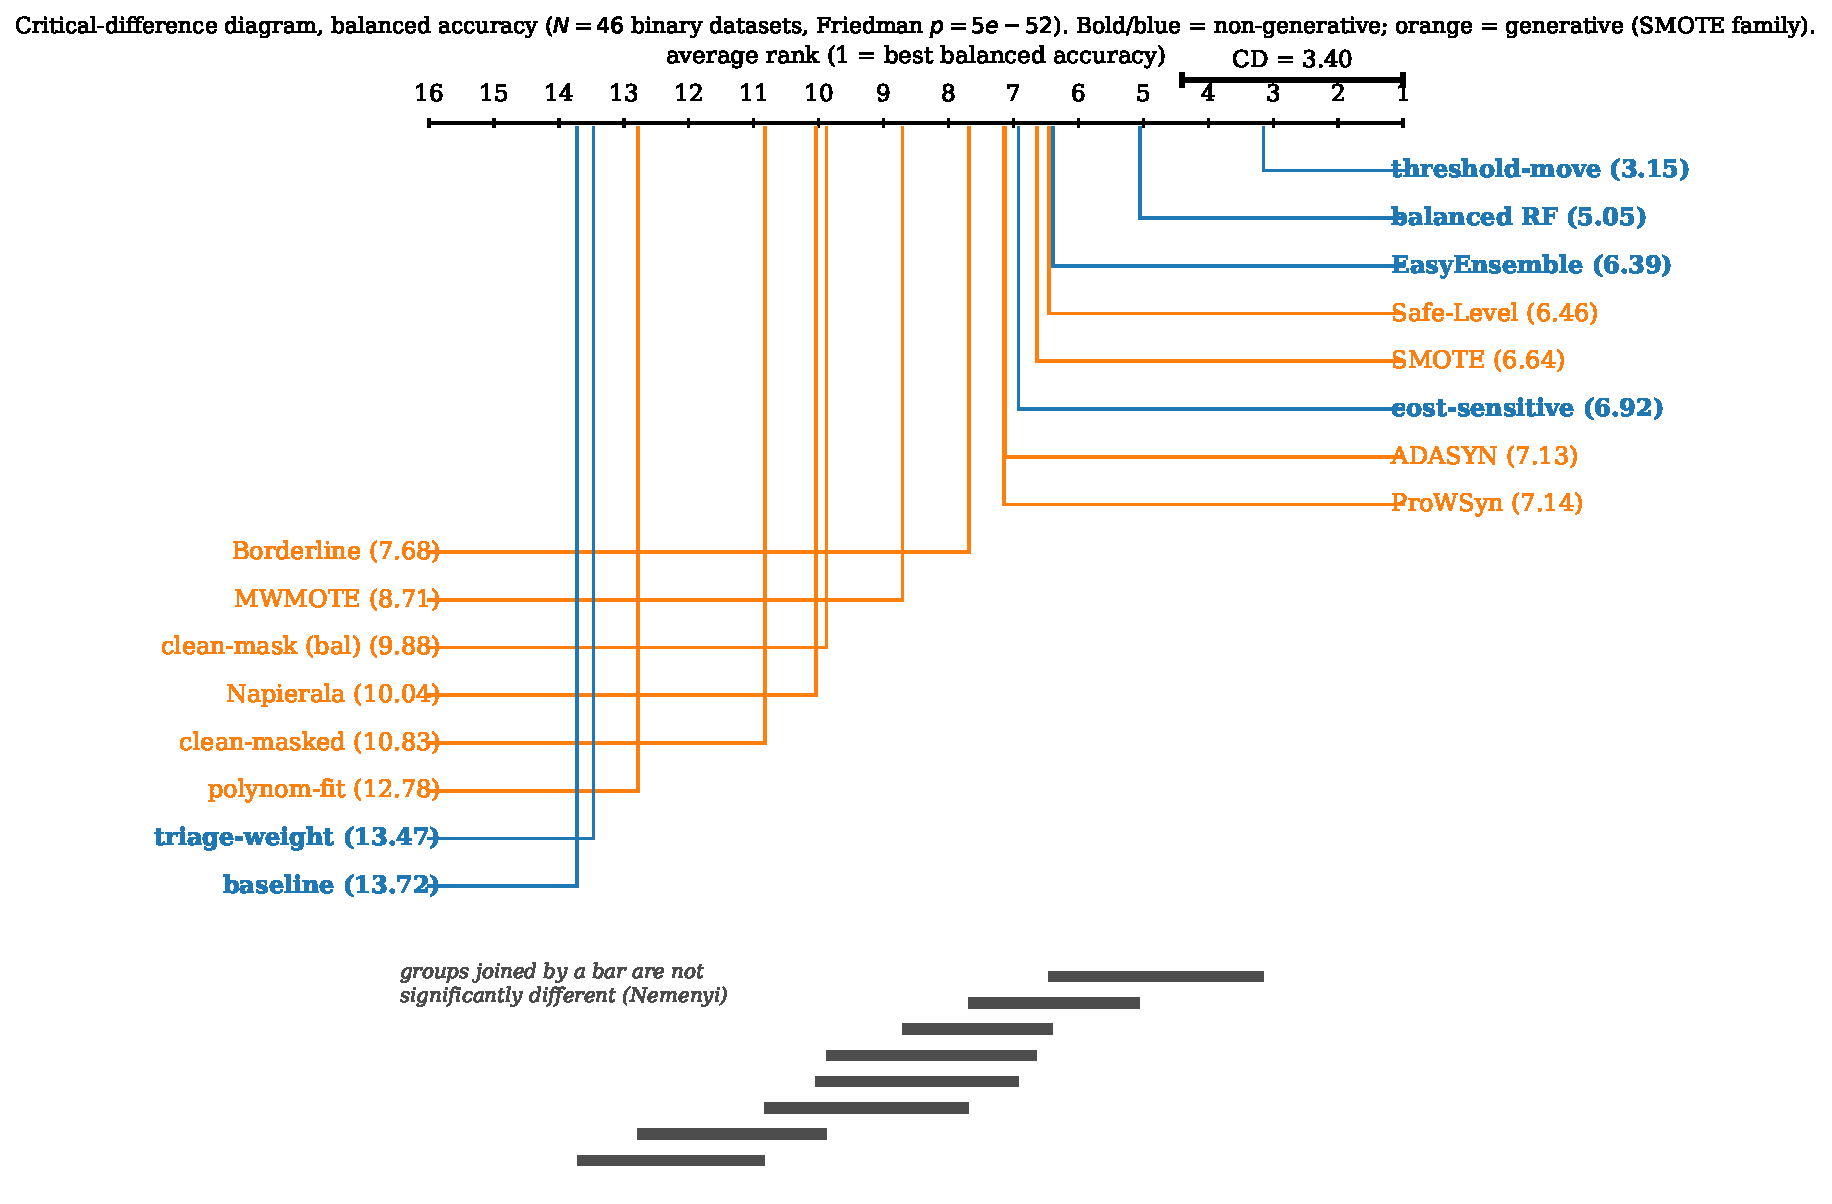
\includegraphics[width=\linewidth]{figures/fig_cd.pdf}
\caption{Critical-difference diagram (Friedman--Nemenyi, $\alpha=0.05$,
$N=46$ binary datasets) of mean per-dataset balanced-accuracy rank over the full
16-strategy menu. Lower rank (right) is better. Non-generative strategies (blue)
threshold-moving, balanced RF, and EasyEnsemble attain the best ranks; the SMOTE
family ranks in the middle; non-rebalancing methods rank worst.}
\label{fig:cd}
\end{figure}

\begin{figure}[t]
\centering
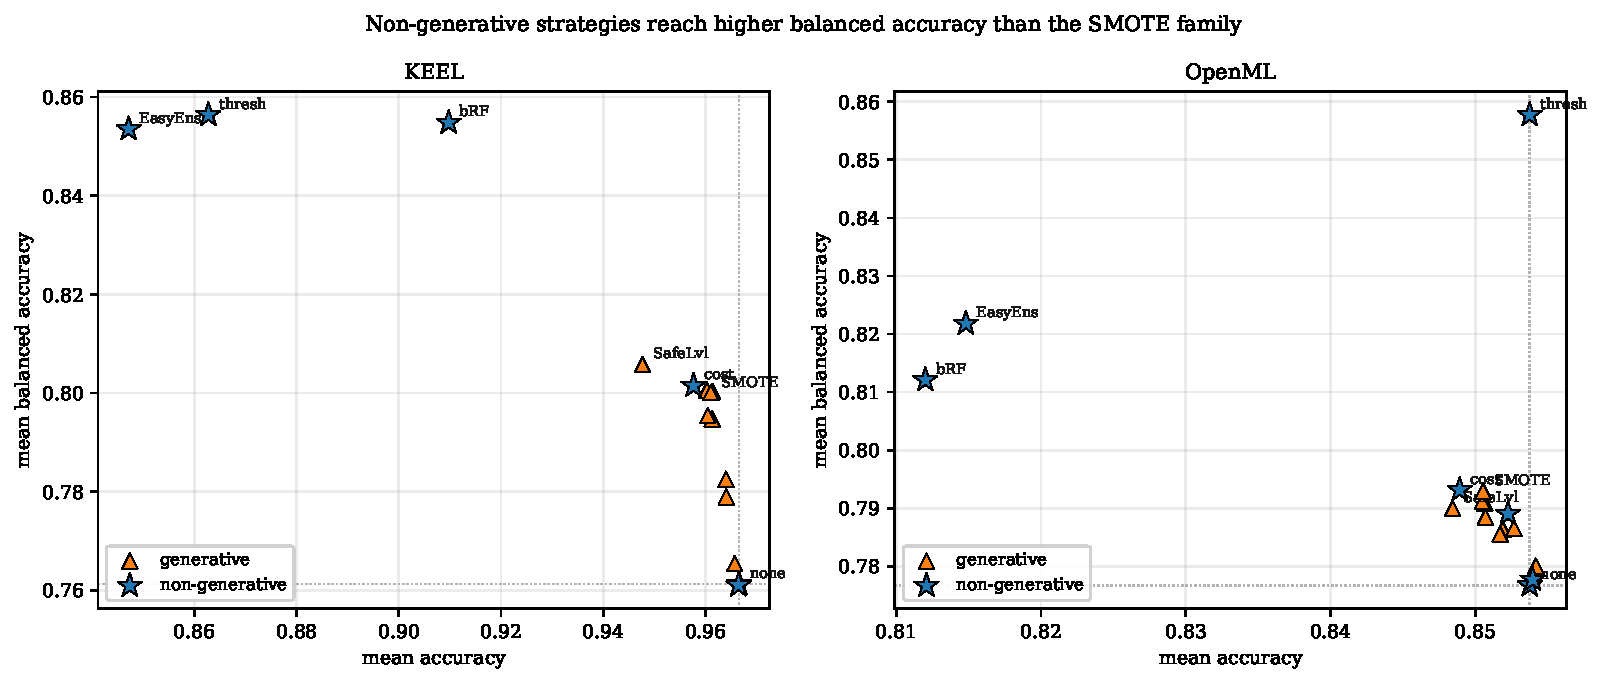
\includegraphics[width=\linewidth]{figures/fig_frontier.pdf}
\caption{Accuracy--balanced-accuracy plane per roster, \emph{at the default
decision threshold}. Non-generative strategies (blue $\star$) reach higher balanced
accuracy than the generative SMOTE family (orange $\triangle$); dotted lines mark
the do-nothing baseline. At threshold parity this gap largely closes
(Table~\ref{tab:parity}).}
\label{fig:frontier}
\end{figure}

\subsection{A regime map: which strategy a dataset needs}\label{sec:results:regime}

\paragraph{Result.} Aggregating the per-dataset oracle choice into five strategy
families, the best move is a balanced ensemble on $42/79$ datasets,
threshold-moving on $17$, cost-sensitive learning on $6$, and \emph{oversampling
on only $12$} ($15\%$); doing nothing is best on $2$. Relative to do-nothing the
mean balanced-accuracy advantage is $+8.1$\,pp for threshold-moving, $+6.1$ for
balanced ensembles, $+3.3$ for oversampling, and $+2.5$ for cost-sensitive
learning. A depth-3 decision tree over the meta-features
(Figure~\ref{fig:regime}) gives an interpretable sketch --- low-separability
(overlapping) data favours balanced ensembles, while large or well-separated data
with a clean minority favours threshold-moving --- but its leave-one-out accuracy
($0.53$) only matches the predict-majority rate, so the map is best read as
\emph{descriptive}: it shows where each family wins, not a rule that beats
``always use a balanced ensemble.''

\begin{figure}[t]
\centering
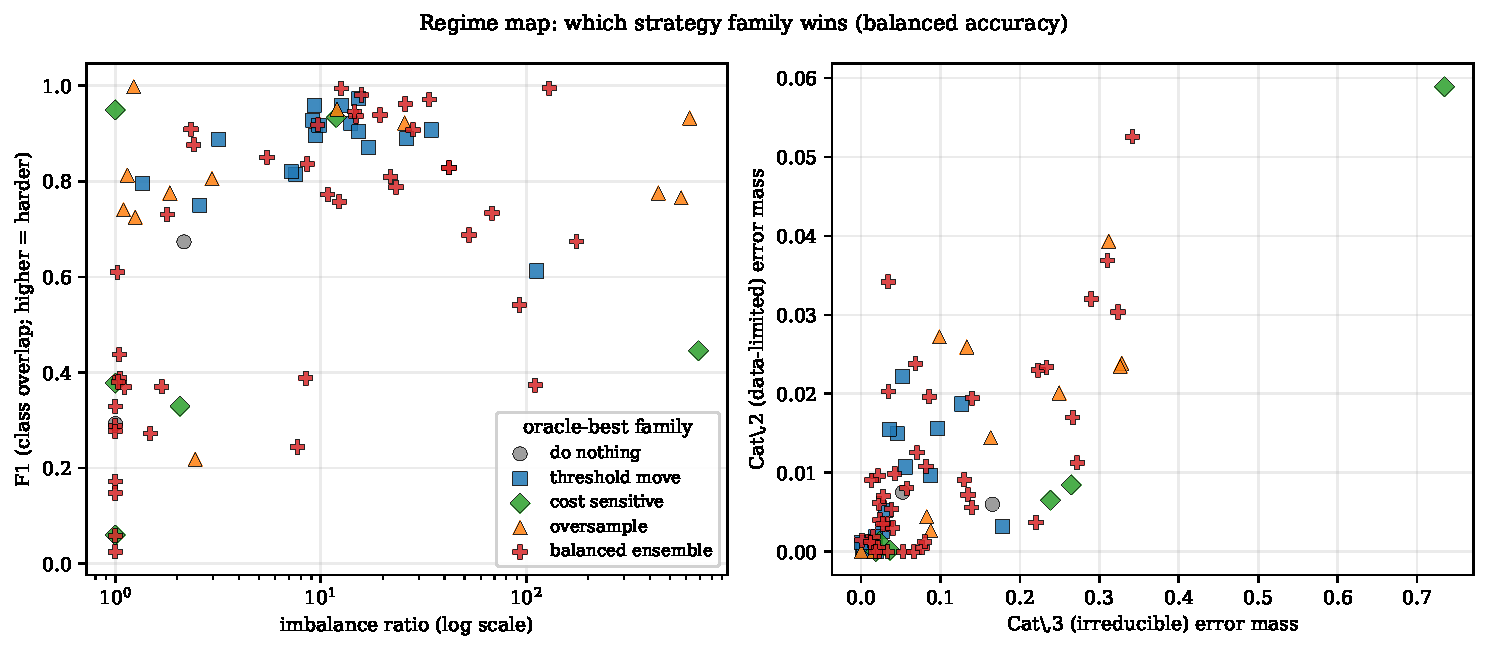
\includegraphics[width=\linewidth]{figures/fig_regime_map.pdf}
\caption{Regime map: the oracle-best strategy family per dataset, over imbalance
ratio vs.\ class overlap (F1, left) and over the triage Cat\,3/Cat\,2 error masses
(right). Oversampling (orange) is best in a minority of regimes; balanced
ensembles and threshold-moving cover most datasets.}
\label{fig:regime}
\end{figure}

\subsection{Prescriptive selection: an honest scope}\label{sec:results:selection}

\paragraph{Result.} Can per-dataset meta-features prescribe the strategy? We train
a leave-one-dataset-out selector on the error-structure and complexity
meta-features and compare it to fixed baselines and an oracle
(Table~\ref{tab:selection}). The selector beats always-SMOTE decisively
($+3.5$\,pp balanced accuracy, $p<10^{-4}$) --- but so does an imbalance-ratio-only
rule, because the gain comes from \emph{having non-generative strategies on the
menu}, not from sophisticated selection. Over the strongest \emph{fixed} strategy
(balanced RF) the edge is real but modest and design-dependent: a direct
method-\emph{classifier} recovers $\sim$60\% of the oracle headroom and robustly
beats best-fixed on balanced accuracy ($+0.64$\,pp, $8/8$ seeds $p\le0.01$) and
G-mean ($+0.64$\,pp, $8/8$ $p\le0.03$), but not MCC; a per-method \emph{regressor}
and the interpretable rule both tie best-fixed.

\begin{table}[t]
\centering
\caption{Prescriptive selection over the full 16-strategy menu, leave-one-dataset-out
across 79 datasets (mean realized metric). A learned selector built on error-structure
and complexity meta-features beats always-SMOTE decisively, but over the strongest
\emph{fixed} strategy its edge is modest: the direct method-classifier robustly beats
best-fixed on balanced accuracy (+0.64\,pp, $8/8$ seeds $p{\le}0.01$) and G-mean
(+0.64\,pp, $8/8$ $p{\le}0.03$) but not MCC; the per-method regressor and an
imbalance-ratio-only rule both tie best-fixed. The dominant lever is the menu, not the
selector.}
\label{tab:selection}
\small
\begin{tabular}{l ccc}
\toprule
Selector / fixed strategy & bal.\ acc & G-mean & MCC \\
\midrule
Oracle (per-dataset best, ceiling)        & 0.838 & 0.866 & 0.696 \\
\midrule
Learned selector --- classifier           & \textbf{0.833} & \textbf{0.862} & 0.677 \\
Learned selector --- regressor            & 0.829 & 0.858 & 0.675 \\
Imbalance-ratio-only selector             & 0.827 & 0.856 & 0.673 \\
\midrule
Best fixed strategy\,$^{a}$               & 0.827 & 0.855 & 0.680 \\
Always-SMOTE                              & 0.795 & 0.827 & 0.678 \\
Baseline (do nothing)                     & 0.772 & 0.805 & 0.670 \\
\bottomrule
\end{tabular}\\[2pt]
{\footnotesize $^{a}$ Best fixed strategy is balanced RF for balanced accuracy and
G-mean, cost-sensitive for MCC.}
\end{table}


\paragraph{Interpretation.} This is a direct, held-out, real-data answer to the
characteristic-driven selection problem left open by \cite{jiang2026beyond}: error-structure
features yield a selector that beats the always-SMOTE paradigm and recovers most
of the achievable gain, but the dominant lever is the \emph{menu}, not selector
sophistication. Indeed, an imbalance-ratio-only selector matches the full
meta-feature selector (Table~\ref{tab:selection}), so the error-structure features
add no measurable \emph{selection} value --- the triage's role here is
explanatory (localizing the boundary for the mechanistic account), not predictive. The
actionable recommendation is therefore simple and robust:
default to a strong non-generative strategy (balanced random forest, or
threshold-moving when calibrated probabilities matter), and reserve oversampling
for the minority of regimes where the map says it wins.

\subsection{Computational cost}\label{sec:results:cost}

The triage (5 forests $\times$ 100 trees) costs $\sim$1\,s on small datasets to
$\sim$33\,s at $n\approx50{,}000$, scaling as $O(n\log n)$ in the training-set size
(dominated by the forest fits; \appref{app:cost}). Crucially it is a \emph{one-time},
classifier-agnostic preprocessing step whose category assignments are reused across
every downstream configuration, fold, and base learner, so over a realistic
model-selection budget it is a small \emph{amortized} cost --- well below the
repeated resample-and-refit it informs, not an added per-model overhead. On very
large datasets the stratified $10{,}000$-instance subsample
(\appref{app:subsampling}) bounds it further without changing the category
distribution, so the triage does not become a bottleneck relative to a single SMOTE
fit.

\section{Discussion}\label{sec:discussion}

\paragraph{The tradeoff is a decision problem, not a data problem.} Our central
finding is that the minority-class deficit \emph{decomposes by remedy} and is
predominantly \emph{threshold-recoverable}: across 79 datasets a mean of $69\%$ of
minority errors ($74\%$ at $\mathrm{IR}>3$) are corrected by moving the decision
threshold alone, with only $\sim$7\% data-reducible and $\sim$16\% irreducible.
This explains a regularity the field has documented but not explained --- that
resampling leaves ranking (AUC) unchanged and a threshold shift reproduces its
benefit without synthetic generation and with better calibration
\cite{provost2000imbalanced,elor2022smote,goorbergh2022harm,dalpozzolo2015calibrating}
--- and reframes the long-observed accuracy/recall tradeoff: oversampling is an
implicit, inefficient enactment of a threshold move (it shifts the operating point
by generating across the overlap boundary, at an accuracy and calibration cost),
not a way to build a better classifier. Consistent with this, once every strategy
is given the same threshold tuning the large default-threshold gap between the
families collapses to within $\pm1$\,pp.

\paragraph{Exclusion vs.\ targeting.} The dominant paradigm in oversampling
research \emph{targets} sparse or boundary regions for generation
(ADASYN \cite{he2008adasyn}, Borderline-SMOTE \cite{han2005borderline}, and a long
tail of variants \cite{kovacs2019smote}). Our mechanism explains why this has not
resolved the tradeoff: these variants all generate at or near the boundary, which
is exactly where generation manufactures majority-territory ``minority'' points.
Consistent with this, masking the boundary seeds from SMOTE removes both the
accuracy cost \emph{and} the balanced-accuracy benefit --- corroborating that the
benefit \emph{is} the boundary generation --- so the productive move is not a
better oversampler but a different lever entirely.

\paragraph{The menu matters more than the selector.} A recent line of work asks
which data characteristics should pick the resampler
\cite{jiang2026beyond,carvalho2025resampling}, but its rules barely beat
always-SMOTE. We find the reason: given a menu that includes the dominant
non-generative strategies, even an imbalance-ratio-only rule beats always-SMOTE,
and a learned selector over rich error-structure and complexity meta-features adds
only a modest, robust increment over the single best fixed strategy (balanced
random forest) --- significant on balanced accuracy and G-mean, absent on MCC. The
practical recommendation is therefore not a sophisticated selector but a change of
default: prefer a strong non-generative strategy, and reserve oversampling for the
$\sim$15\% of regimes where the map (\S\ref{sec:results:regime}) says it
wins.

\paragraph{Relation to prior categorization and complexity work.} Napiera{\l}a
\& Stefanowski's instance types \cite{napierala2016types} and data-complexity
measures \cite{komorniczak2022data,santos2023unifying} characterize imbalanced
problems descriptively, and meta-learning relates those characteristics to
observed performance \cite{carvalho2025resampling}. Our contribution is
orthogonal and mechanism-level: the aleatoric--epistemic decomposition localizes
the boundary/overlap region, and the interventional design probes \emph{why}
boundary generation hurts, rather than reporting a correlation. This
intervention-supported account is what the otherwise extensive selection
literature lacks.

\paragraph{Toward deep imbalanced learning.} Our base learners are tabular
(gradient-boosted trees, random forests, logistic regression); the analysis is
deliberately a controlled, mechanism-level foundation laid before the deep case. Two
of its three pillars are architecture-agnostic, and we expect them to carry over. The
remedy decomposition needs only a ranking score and an aleatoric--epistemic signal,
both available from deep models via deep ensembles or MC-dropout
\cite{lakshminarayanan2017simple}; and the threshold-recoverability result is the same
operating-point logic that already explains why imbalanced-trained neural networks are
systematically miscalibrated and recover under post-hoc threshold/temperature
adjustment \cite{guo2017calibration}. The boundary-generation mechanism is the part
that needs care: deep oversampling typically interpolates in a \emph{learned latent}
space rather than the input space (e.g.\ DeepSMOTE \cite{dablain2022deepsmote}), so
Proposition~\ref{prop:cross} would apply to the \emph{latent} posterior, whose geometry
the encoder itself shapes. We therefore present these results as the necessary tabular
proof-of-mechanism and offer a concrete, testable hypothesis: latent-space
interpolation across the embedded decision boundary should reproduce the same
accuracy/recall tradeoff, and a latent threshold move should likewise recover most of
the minority deficit. Testing it across architectures is the natural next thread.

\paragraph{Limitations.} (i) The learned selector's edge over a strong fixed
default is small ($\sim$0.6\,pp) and metric-dependent (present on balanced
accuracy and G-mean, absent on MCC); we report it honestly rather than as a
headline, and conclude that a fixed non-generative default is the pragmatic
recommendation. (ii) The triage thresholds ($\tau_{\text{noise}}=0.12$,
$\tau_{\text{cat2}}=0.4$) are fixed across datasets; a sensitivity analysis
(\appref{app:sensitivity}) shows category assignments and downstream
accuracy are stable across a wide range. (iii) We validate the default-threshold
advantage --- and its collapse to within $\pm1$\,pp at threshold parity --- across
three tabular base learners (gradient-boosted trees, random forests, and logistic
regression; \S\ref{sec:results:frontier}), so neither the default-threshold gap nor
the operating-point explanation is a model-specific artefact; the extension to
\emph{deep} imbalanced learning is its own thread, sketched above. (iv) The regime map is descriptive: a depth-3 rule does not beat
``always use a balanced ensemble,'' so the map informs rather than automates the
choice.

\section{Conclusion}\label{sec:conclusion}

We introduced a remedy decomposition of the misclassified minority class that sorts
each error into \emph{threshold-recoverable}, \emph{data-reducible} (epistemic), or
\emph{irreducible} (aleatoric), and used it to explain why class-imbalance
correction so often reduces to a decision-threshold change. Across 79 real datasets
the minority deficit is overwhelmingly threshold-recoverable (mean $69\%$, $74\%$ at
imbalance ratio $>3$): the classifier already ranks these instances correctly and
only the default cutoff is wrong. This accounts mechanistically for a documented but
unexplained regularity, namely that SMOTE-family oversampling does not improve ranking
and a threshold
move reproduces its benefit without synthetic generation or probability
distortion, and
recasts the long-observed accuracy/recall tradeoff as an operating-point effect:
such oversampling is an implicit, inefficient enactment of a threshold shift, which on
controlled data we show it achieves by generating across the overlap boundary. Once
every strategy is given the same out-of-fold threshold tuning, the large
default-threshold gap between the families collapses to within $\pm1$\,pp across
three base learners (six evaluated; naive Bayes shows a small but significant
generative edge of $1.6$\,pp, and the single undertrained MLP, whose ranking
imbalance itself corrupts, marks the account's boundary). The
decomposition also says \emph{when} the threshold is not enough: the small
data-reducible fraction is where minority data genuinely helps, the irreducible
fraction where no remedy in our menu does, though a strong non-generative default is
near-optimal in the threshold-recoverable majority. The practical message is simple:
diagnose the deficit, and for most of it, move the decision rather than oversample.


\appendix

\section{Threshold Sensitivity}\label{app:sensitivity}

The triage thresholds ($\tau_{\text{noise}} = 0.12$, $\tau_{\text{cat2}} = 0.4$)
and the triage-weighting upweight factor ($w = 2.0$, the sample-weight multiplier
that the triage-weighting strategy of \S\ref{sec:method:menu} applies to the correct
same-class neighbours of Cat\,2 errors) are fixed across all datasets. We swept each threshold across a
range of values and measured downstream XGBoost accuracy: $\tau_{\text{noise}}
\in [0.05, 0.30]$, $\tau_{\text{cat2}} \in [0.2, 0.6]$, $w \in [1.0, 5.0]$.
Across the benchmark datasets, 74\% show $< 0.5\%$ accuracy
variation across all configurations, supporting the use of fixed thresholds
as a sensible default. The two methods (clean-masked SMOTE, triage
weighting) maintain their relative ordering vs.\ baselines at every threshold
configuration tested.

\section{Out-of-Fold Triage Validation}\label{app:oof}

The triage categories underpin the mechanistic argument (\S\ref{sec:results:interventional}),
so we verify they are not optimistic in-sample artefacts. Two facts establish this.
First, by construction every model-derived signal that drives the categorization is
\emph{out-of-bag}: the error indicator is the OOB ensemble majority vote, and the
true-class probability is the OOB estimate (\S\ref{sec:method:uncert}); the only
non-model signal, the local class ratio, is a property of the data geometry.
Second, as a strict check we re-derive the categories under inner $5$-fold
cross-validation: forests fit on the inner-training folds categorize the held-out
instances (via held-out predictions for the error indicator, true-class
probability, and the full aleatoric/epistemic decomposition; neighbour-based
signals are measured against the inner-training set). Over the 79 datasets, the
Cat\,3 (irreducible) fraction among errors is essentially unchanged: the in-sample
and out-of-fold means coincide at $0.838$, the per-dataset Spearman correlation is
$0.97$ ($p<10^{-40}$), and the mean absolute shift is $\OOFCATSHIFT$\,pp (median
$1.0$\,pp). The aleatoric/epistemic ordering that motivates the categories is
preserved out-of-fold (Cat\,3 aleatoric uncertainty exceeds Cat\,2's on $80\%$ of
datasets). The category \emph{identification} is therefore not an in-sample
artefact. We note separately that the small real-data \emph{interventional} effect
(\S\ref{sec:results:interventional}) is sensitive to this re-estimation: with
out-of-fold seeds and a reduced $3\times3$ protocol the targeted-augmentation
contrast remains directionally consistent (random augmentation null) but is no
longer individually significant, which is why we rest the mechanism on the
controlled experiment (\S\ref{sec:results:mechanism}) and the
discrimination/threshold analysis (\S\ref{sec:results:frontier}) rather than on the
real-data intervention.

\section{GBM Triage Agreement}\label{app:gbm}

To verify that the three-way decomposition is not specific to random
forests, we replaced the RF ensemble with bagged XGBoost (5 bags of 100
trees, matching the RF configuration). On a 20-dataset agreement subset,
the GBM-based triage assigns 82\% of training instances to the same category
as the RF-based triage. Downstream accuracy under both triages is
comparable (mean absolute difference $0.04\%$), indicating that any
ensemble model exposing per-tree predictions can drive the decomposition.

\section{Subsampling Category-Structure Control}\label{app:subsampling}

We verified that stratified subsampling to 10\,000 instances preserves the
triage category distribution. On the five largest datasets in our
benchmark, we computed the per-category fraction $\{p_{\text{correct}},
p_{\text{noise}}, p_{\text{data-limited}}, p_{\text{irreducible}}\}$ on the
full dataset and on a single stratified 10\,000-instance subsample. The
mean absolute deviation between the two distributions is $< 2$ percentage
points per category across all five datasets, validating the subsampling
protocol used throughout (\S\ref{sec:results:frontier}).
Detailed per-dataset numbers are provided in the supplementary material.

\section{Computational Cost Detail}\label{app:cost}

Full cost-table breakdown by dataset (extending \S\ref{sec:results:cost}):

\begin{table}[t]
\centering
\caption{Triage wall-clock cost vs.\ a single XGBoost fit (mean over repeats). Overhead = triage time as a percentage of total pipeline time. The triage is a one-time, classifier-agnostic preprocessing cost.}
\label{tab:cost}
\begin{tabular}{lrrrrr}
\toprule
Dataset & $n$ & $d$ & Triage (s) & XGB (s) & Overhead (\%) \\
\midrule
\texttt{iris} & 150 & 4 & 1.04 & 0.15 & 87.2 \\
\texttt{wine} & 178 & 13 & 1.31 & 0.08 & 94.1 \\
\texttt{sonar} & 208 & 60 & 1.10 & 0.12 & 90.2 \\
\texttt{glass} & 214 & 9 & 1.17 & 0.96 & 64.8 \\
\texttt{ionosphere} & 351 & 34 & 1.05 & 0.12 & 89.9 \\
\texttt{vehicle} & 846 & 18 & 1.27 & 0.40 & 76.1 \\
\texttt{vowel} & 990 & 12 & 1.91 & 1.59 & 56.0 \\
\texttt{credit-g} & 1000 & 20 & 1.43 & 0.16 & 89.8 \\
\texttt{segment} & 2310 & 19 & 1.56 & 0.93 & 63.4 \\
\texttt{phoneme} & 5404 & 5 & 2.71 & 0.74 & 77.6 \\
\texttt{satimage} & 6430 & 36 & 2.87 & 2.19 & 58.5 \\
\texttt{eeg-eye-state} & 14980 & 14 & 10.20 & 0.60 & 94.6 \\
\texttt{MagicTelescope} & 19020 & 10 & 8.40 & 1.25 & 88.8 \\
\texttt{bank-marketing} & 45211 & 16 & 16.79 & 0.84 & 95.6 \\
\texttt{covertype} & 50000 & 54 & 32.63 & 49.05 & 50.1 \\
\bottomrule
\end{tabular}
\end{table}


The triage time scales roughly as $O(n \log n)$ in the number of training
instances and is dominated by the random-forest fits; the local class-ratio
computation (k-NN with $k=5$) contributes $< 5\%$ of total triage time
across all dataset sizes.

\section{Instrument Robustness: Non-Tree Ensembles}\label{app:nontree}

The remedy decomposition's model-derived signals come from a random-forest
ensemble (\S\ref{sec:method:uncert}). To verify the headline is not an
artefact of tree-based uncertainty, we re-derive the full decomposition with
two bagged non-tree instruments over the full 27 KEEL + 54
OpenML/scikit-learn roster (81 dataset cells; the headline statistics of
Table~\ref{tab:reducibility} use the 79-dataset menu roster of \S\ref{sec:design}): $B{=}25$
bootstrap-bagged multilayer perceptrons (scaled, $64{\times}32$ hidden units,
early stopping) and $B{=}25$ bootstrap-bagged logistic regressions. Every
signal remains out-of-bag: only ensemble members whose bootstrap excluded an
instance contribute to its probabilities, and the Shaker-style
aleatoric--epistemic decomposition is taken over those members. The local
class ratio is the identical $k$-NN computation, and the error set, one-vs-rest
intervention, and cross-fitted threshold follow \S\ref{sec:method:remedy}
exactly. Two design notes: (i)~members
are unweighted, matching the headline instrument (\S\ref{sec:method:remedy}) ---
class-balanced members enact the operating-point shift
\emph{inside} the instrument (completely so for logistic regression,
\S\ref{sec:results:frontier}) and dissolve the default-threshold deficit being
decomposed; (ii)~Cat\,1 is gated by TCP alone, as the forest-consensus noise
score has no non-tree analogue, which shifts part of the residue from the
data-reducible/irreducible classes into noise but leaves the
threshold-recoverability axis untouched.

\begin{table}[t]
\centering
\caption{Remedy decomposition by instrument (means over datasets with
$\ge 5$ minority errors; definitions of \S\ref{sec:method:remedy}). The
threshold-recoverable share, the paper's headline, is stable across
instruments; the per-dataset correlation with the RF instrument is given in
the last column. The non-tree instruments assign more of the residue to noise
(TCP-only gate, note (ii)).}
\label{tab:nontree}
\footnotesize
\begin{tabular}{lrrrrrr}
\toprule
Instrument & thr.-rec. & (median) & data-red. & irred. & noise & $r$ vs RF \\
\midrule
Random forests (paper instrument) & 69\% & (75\%) & 7\% & 16\% & 7\% & --- \\
Bagged MLPs & 69\% & (70\%) & 3\% & 11\% & 18\% & 0.68 \\
Bagged logistic regression & 68\% & (74\%) & 1\% & 10\% & 21\% & 0.55 \\
\bottomrule
\end{tabular}

\end{table}

Threshold-recoverable remains the dominant remedy class under both non-tree
instruments (Table~\ref{tab:nontree}): $62\%$ for bagged MLPs and $63\%$ for
bagged logistic regression against $68\%$ for the RF instrument, rising to
$73\%$ on $\mathrm{IR}>3$ datasets for both (RF: $80\%$), with per-dataset
correlations of $r=0.78$ and $0.72$ against the forest instrument. Part of the
gap to the RF share is the TCP-only noise gate of note (ii), which absorbs
$19$--$24\%$ of the residue into noise. The decomposition's ordering,
threshold-recoverable far above every other remedy class, is
instrument-independent.

\section{Ensemble-Size Sensitivity}\label{app:msens}

The instrument uses $M{=}5$ forests of $T{=}100$ trees, matching standard
deep-ensemble practice ($M{=}5$ in \cite{lakshminarayanan2017simple}).
Recomputing the full decomposition for $M \in \{1,2,5,10,20\}$ on a
10-dataset IR-spanning subset (Table~\ref{tab:msens}): the triage category
fractions move by at most $2.6$\,pp between $M{=}5$ and $M{=}20$, and the
threshold-recoverable share by $3.3$\,pp on average ($1.9$\,pp for $M{=}10$);
the largest single-dataset deviations occur where the minority error set is
tiny (a handful of instances, so one flip moves the fraction by many points).
Below $M{=}5$ the decomposition is visibly unstable (single-dataset swings up
to $34$\,pp). $M{=}5$ therefore sits at
the stability knee, and the conclusions do not change with a larger ensemble.

\begin{table}[t]
\centering
\caption{Ensemble-size sensitivity: mean threshold-recoverable share and
absolute deviations from the $M{=}5$ reference across 10 datasets.}
\label{tab:msens}
\footnotesize
\begin{tabular}{lrrrr}
\toprule
$M$ & mean thr.-rec. & mean $|\Delta$thr.-rec.$|$ & max $|\Delta$thr.-rec.$|$ & max $|\Delta$cat.\ fraction$|$ \\
\midrule
1 & 66\% & 9.4\,pp & 28.6\,pp & 6.4\,pp \\
2 & 71\% & 7.0\,pp & 42.9\,pp & 7.5\,pp \\
5 (ref.) & 70\% & 0.0\,pp & 0.0\,pp & 0.0\,pp \\
10 & 68\% & 3.7\,pp & 11.2\,pp & 2.3\,pp \\
20 & 69\% & 2.3\,pp & 6.2\,pp & 2.3\,pp \\
\bottomrule
\end{tabular}

\end{table}

\section{Extended Oversampler Comparison}\label{app:oversamplers}

Table~\ref{tab:smote} reports the full oversampler family, including the
Kov\'acs top-ranked variants and Geometric SMOTE (added at review), against
standard SMOTE on the OpenML roster.

\begin{table}[t]
\centering
\caption{Oversampler family vs.\ standard SMOTE (XGBoost, 52 OpenML-roster datasets): mean metric, win rate over SMOTE, and Wilcoxon $p$. The geometric variant G-SMOTE (added at review) buys significantly \emph{less} balanced accuracy than SMOTE at a comparable accuracy level; only polynom-fit (a known weak-tradeoff variant) and the triage clean-masked variant significantly recover accuracy.}
\label{tab:smote}
\begin{tabular}{lrrrrrr}
\toprule
Method (vs.\ SMOTE) & Mean Acc & WR Acc & $p_{\text{Acc}}$ & Mean BAcc & WR BAcc & $p_{\text{BAcc}}$ \\
\midrule
baseline & 0.8538 & 53.8\% & 0.001** & 0.7768 & 11.5\% & 0.000*** \\
borderline\_smote & 0.8505 & 38.5\% & 0.914 & 0.7911 & 25.0\% & 0.013* \\
adasyn & 0.8507 & 26.9\% & 0.180 & 0.7909 & 32.7\% & 0.444 \\
safe\_level\_smote & 0.8484 & 36.5\% & 0.379 & 0.7900 & 34.6\% & 0.282 \\
polynom\_fit\_smote & 0.8542 & 55.8\% & 0.001*** & 0.7800 & 17.3\% & 0.000*** \\
prowsyn & 0.8527 & 48.1\% & 0.128 & 0.7866 & 21.2\% & 0.000*** \\
mwmote & 0.8517 & 38.5\% & 0.771 & 0.7856 & 28.8\% & 0.001** \\
gsmote & 0.8510 & 44.2\% & 0.677 & 0.7814 & 25.0\% & 0.000*** \\
napierala\_guided\_smote & 0.8507 & 51.9\% & 0.103 & 0.7885 & 32.7\% & 0.036* \\
clean\_masked\_smote & 0.8519 & 46.2\% & 0.016* & 0.7863 & 17.3\% & 0.000*** \\
\bottomrule
\end{tabular}
\end{table}


\clearpage
\section{Dataset Listing}\label{app:datasets}

Table~\ref{tab:datasets} lists the OpenML/scikit-learn roster, including
each dataset's OpenML ID, number of instances, features, classes, and imbalance
ratio (majority-class count divided by minority-class count); the remaining 27
datasets are the standard \texttt{imbalanced-learn}/KEEL benchmark suite.

\begin{longtable}{lrrrrc}
\caption{Full dataset listing (54 datasets; the recovered original-paper roster). $n$ = instances; $d$ = features; $C$ = classes; IR = imbalance ratio (majority / minority count). ``sklearn'' marks datasets loaded from scikit-learn rather than OpenML; \texttt{webpage}'s class statistics are not reported because its sparse high-dimensional format excludes it from the menu evaluation (\S\ref{sec:design}).}\label{tab:datasets}\\
\toprule
Dataset & OpenML ID & $n$ & $d$ & $C$ & IR \\
\midrule
\endfirsthead
\multicolumn{6}{l}{\tablename~\thetable\ -- continued}\\
\toprule
Dataset & OpenML ID & $n$ & $d$ & $C$ & IR \\
\midrule
\endhead
\midrule \multicolumn{6}{r}{\textit{continued on next page}}\\
\endfoot
\bottomrule
\endlastfoot
\texttt{phoneme} & 1489 & 5404 & 5 & 2 & 2.4 \\
\texttt{electricity} & 151 & 45312 & 8 & 2 & 1.4 \\
\texttt{bank-marketing} & 1461 & 45211 & 16 & 2 & 7.5 \\
\texttt{MagicTelescope} & 1120 & 19020 & 10 & 2 & 1.8 \\
\texttt{MiniBooNE} & 41150 & 50000 & 50 & 2 & 2.6 \\
\texttt{jannis} & 41168 & 50000 & 54 & 4 & 23.2 \\
\texttt{covertype} & 1596 & 50000 & 54 & 7 & 109.5 \\
\texttt{credit-g} & 31 & 1000 & 20 & 2 & 2.3 \\
\texttt{vehicle} & 54 & 846 & 18 & 4 & 1.1 \\
\texttt{segment} & 36 & 2310 & 19 & 7 & 1.0 \\
\texttt{kc1} & 1067 & 2109 & 21 & 2 & 5.5 \\
\texttt{pc4} & 1049 & 1458 & 37 & 2 & 7.2 \\
\texttt{ozone-level-8hr} & 1487 & 2534 & 72 & 2 & 14.8 \\
\texttt{sick} & 38 & 3772 & 29 & 2 & 15.3 \\
\texttt{abalone} & 183 & 4177 & 8 & 28 & 689.0 \\
\texttt{yeast} & 181 & 1484 & 8 & 10 & 92.6 \\
\texttt{oil\_spill} & 1018 & 8844 & 56 & 2 & 14.6 \\
\texttt{mammography} & 310 & 11183 & 6 & 2 & 42.0 \\
\texttt{wine\_quality} & 287 & 6497 & 11 & 7 & 567.2 \\
\texttt{thyroid} & 40474 & 2800 & 26 & 5 & 52.6 \\
\texttt{satimage} & 182 & 6430 & 36 & 6 & 2.4 \\
\texttt{creditcard} & 1597 & 50000 & 29 & 2 & 601.4 \\
\texttt{webpage} & 350 & 34780 & 300 & -- & -- \\
\texttt{solar-flare} & 40687 & 1066 & 12 & 6 & 7.7 \\
\texttt{iris} & sklearn & 150 & 4 & 3 & 1.0 \\
\texttt{wine} & sklearn & 178 & 13 & 3 & 1.5 \\
\texttt{breast\_cancer} & sklearn & 569 & 30 & 2 & 1.7 \\
\texttt{digits} & sklearn & 1797 & 64 & 10 & 1.1 \\
\texttt{glass} & 41 & 214 & 9 & 6 & 8.4 \\
\texttt{vowel} & 307 & 990 & 12 & 11 & 1.0 \\
\texttt{letter} & 6 & 20000 & 16 & 26 & 1.1 \\
\texttt{optdigits} & 28 & 5620 & 64 & 10 & 1.0 \\
\texttt{page-blocks} & 30 & 5473 & 10 & 5 & 175.5 \\
\texttt{sonar} & 40 & 208 & 60 & 2 & 1.1 \\
\texttt{eeg-eye-state} & 1471 & 14980 & 14 & 2 & 1.2 \\
\texttt{waveform} & 60 & 5000 & 40 & 3 & 1.0 \\
\texttt{madelon} & 1485 & 2600 & 500 & 2 & 1.0 \\
\texttt{GesturePhaseSegmentationProcessed} & 4538 & 9873 & 32 & 5 & 3.0 \\
\texttt{JapaneseVowels} & 375 & 9961 & 14 & 9 & 2.1 \\
\texttt{heart-statlog} & 53 & 270 & 13 & 2 & 1.2 \\
\texttt{ionosphere} & 59 & 351 & 34 & 2 & 1.8 \\
\texttt{wine-quality-white} & 40498 & 4898 & 11 & 7 & 439.6 \\
\texttt{wine-quality-red} & 40691 & 1599 & 11 & 6 & 68.1 \\
\texttt{mfeat-factors} & 12 & 2000 & 216 & 10 & 1.0 \\
\texttt{mfeat-fourier} & 14 & 2000 & 76 & 10 & 1.0 \\
\texttt{mfeat-karhunen} & 16 & 2000 & 64 & 10 & 1.0 \\
\texttt{mfeat-morphological} & 18 & 2000 & 6 & 10 & 1.0 \\
\texttt{mfeat-pixel} & 20 & 2000 & 240 & 10 & 1.0 \\
\texttt{mfeat-zernike} & 22 & 2000 & 47 & 10 & 1.0 \\
\texttt{semeion} & 1501 & 1593 & 256 & 10 & 1.0 \\
\texttt{synthetic\_control} & 377 & 600 & 60 & 6 & 1.0 \\
\texttt{adult} & 179 & 48842 & 14 & 2 & 3.2 \\
\texttt{splice} & 46 & 3190 & 60 & 3 & 2.2 \\
\texttt{USPS} & 41082 & 9298 & 256 & 10 & 2.2 \\
\end{longtable}



\section*{CRediT authorship contribution statement}

\textbf{Cameron Hamilton:} Conceptualization, Methodology, Software, Formal
analysis, Investigation, Data curation, Writing -- original draft, Writing --
review \& editing, Visualization.

\section*{Declaration of competing interest}

The authors declare that they have no known competing financial interests or
personal relationships that could have appeared to influence the work reported in
this paper.

\section*{Funding}

This research did not receive any specific grant from funding agencies in the
public, commercial, or not-for-profit sectors.

\section*{Data availability}

All datasets are publicly available (the \texttt{imbalanced-learn}/KEEL benchmark
suite and OpenML). Code, runner scripts, result files, and a one-command
reproduction guide are publicly available at
\url{https://github.com/allianceai/eit}.

\section*{Declaration of generative AI and AI-assisted technologies in the manuscript preparation process}

During the preparation of this work the author used Anthropic's Claude and the
Claude Code assistant in order to draft and edit manuscript text, improve language
and structure, assist with literature search and \LaTeX{} formatting, and produce
figures, diagrams, and tables from the author's own data and analyses. After using
these tools, the author reviewed and edited all content, independently verified the
results, statistical claims, and cited references, and takes full responsibility for
the content of the published article.


\bibliographystyle{elsarticle-num}
\bibliography{references}

\end{document}
